\documentclass[9pt]{beamer}

\usepackage[utf8]{inputenc}
\usepackage[T1]{fontenc}

\usepackage{longtable}
\usepackage{booktabs}

\usepackage{graphicx}
\usepackage{subfig}
\usepackage{floatrow}
\captionsetup{labelsep=period}

\usepackage{tikz}
\usetikzlibrary{arrows}

\usepackage{standalone}

\usepackage{amssymb}
\usepackage{amsmath}
\usepackage{mathrsfs}
\usepackage{mathtools}
\usepackage{dsfont}
\usepackage{bbold}
\usepackage{breqn}


\usepackage{pdfpages}
\usepackage{hyperref}

\usepackage{color}


\usetheme{ign}

\title{Traitements avancés des images de Télédétection}
\subtitle{SVM et Sélection d'attribut}
\author{Oussama ENNAFII}
\institute{ENSG}
\date{\today}

\begin{document}

	\begin{frame}[plain]
		\titlepage{}
	\end{frame}

	\section{Introduction}

	\begin{frame}{Rappel}
		\begin{figure}[H]
			\begin{center}
				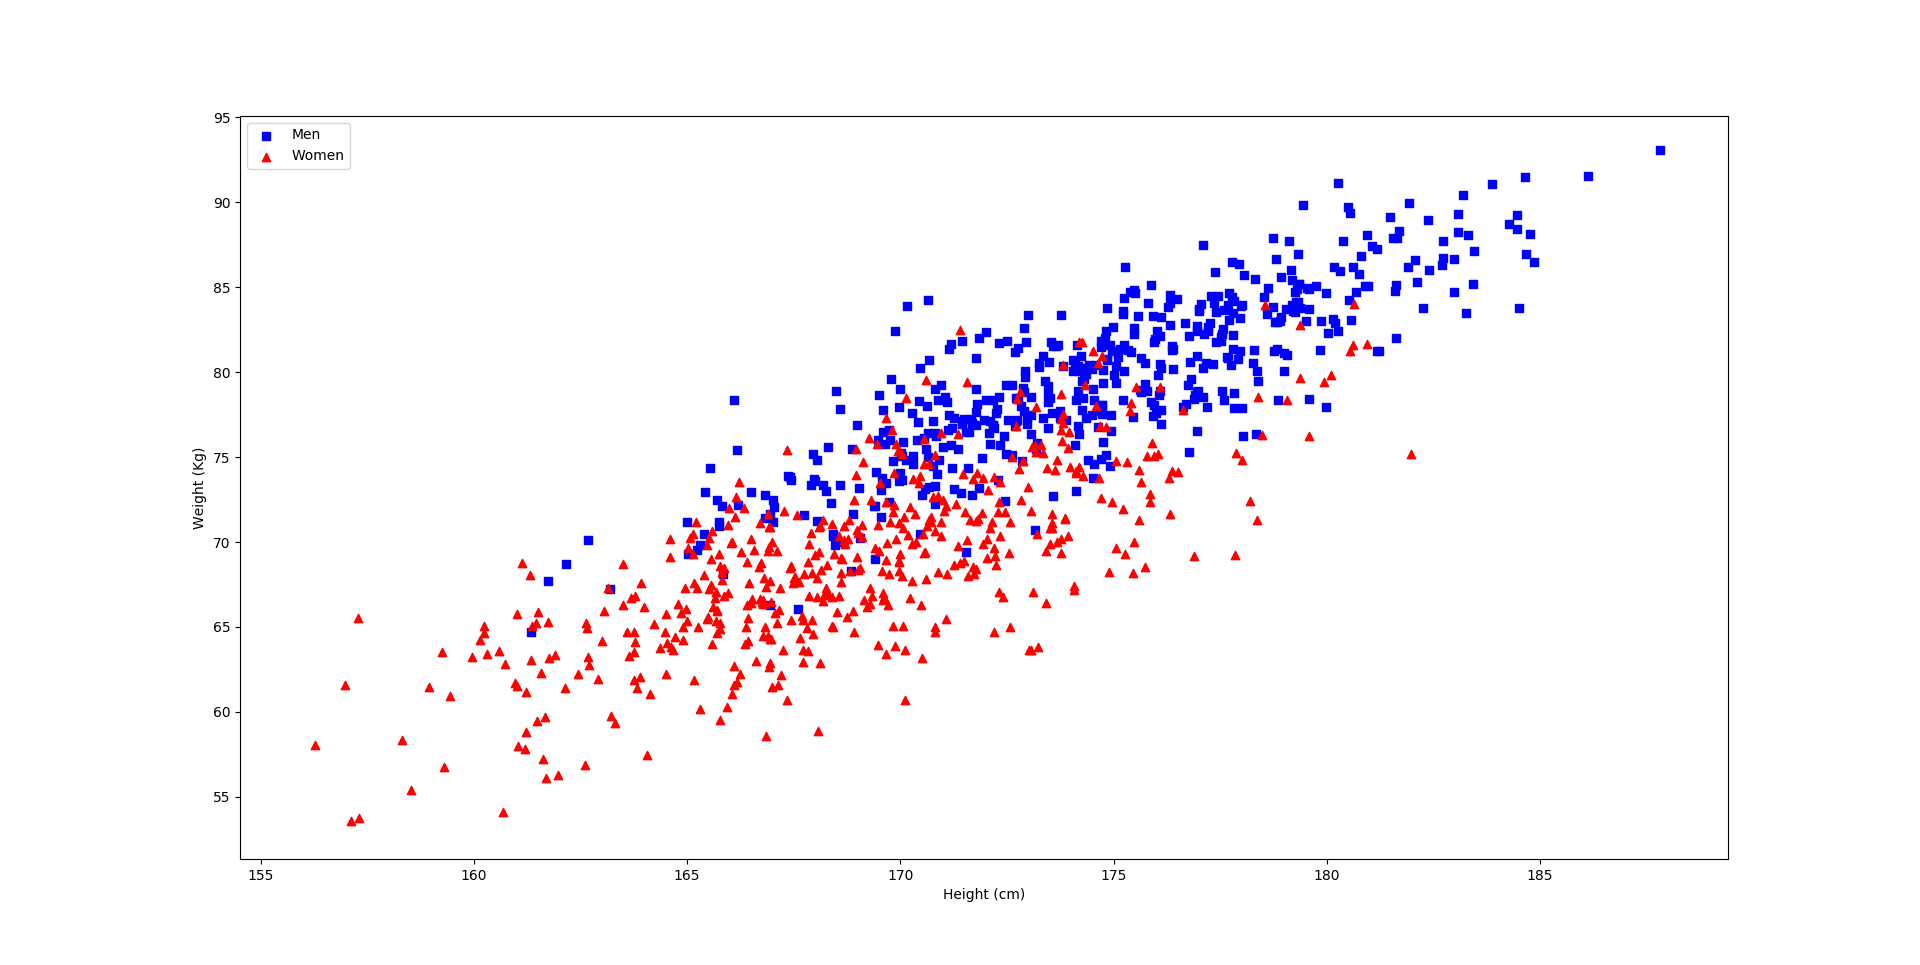
\includegraphics[width=.7\textwidth]{images/samples/sample_2d}
				\caption{\label{fig::sample_2d} Exemple de problème de classification: $2$ attributs et $2$ classes.}
			\end{center}
		\end{figure}
		\begin{itemize}
			\item[--]<1-> On observe $n$ échantillons: $\Big((X^i, Y^i)\Big)_{i=1,\dots,n}$,
			\item[--]<2-> Sachant une instance $X^j = \begin{pmatrix}
			X_1^j\\
			\vdots \\
			X_d^j
			\end{pmatrix}$, il faut prédire sa classe $Y^j$ et sa probabilité.
		\end{itemize}
	\end{frame}

	\begin{frame}{Supervisé vs Non-Supervisée}
		\begin{figure}[H]
			\begin{center}
				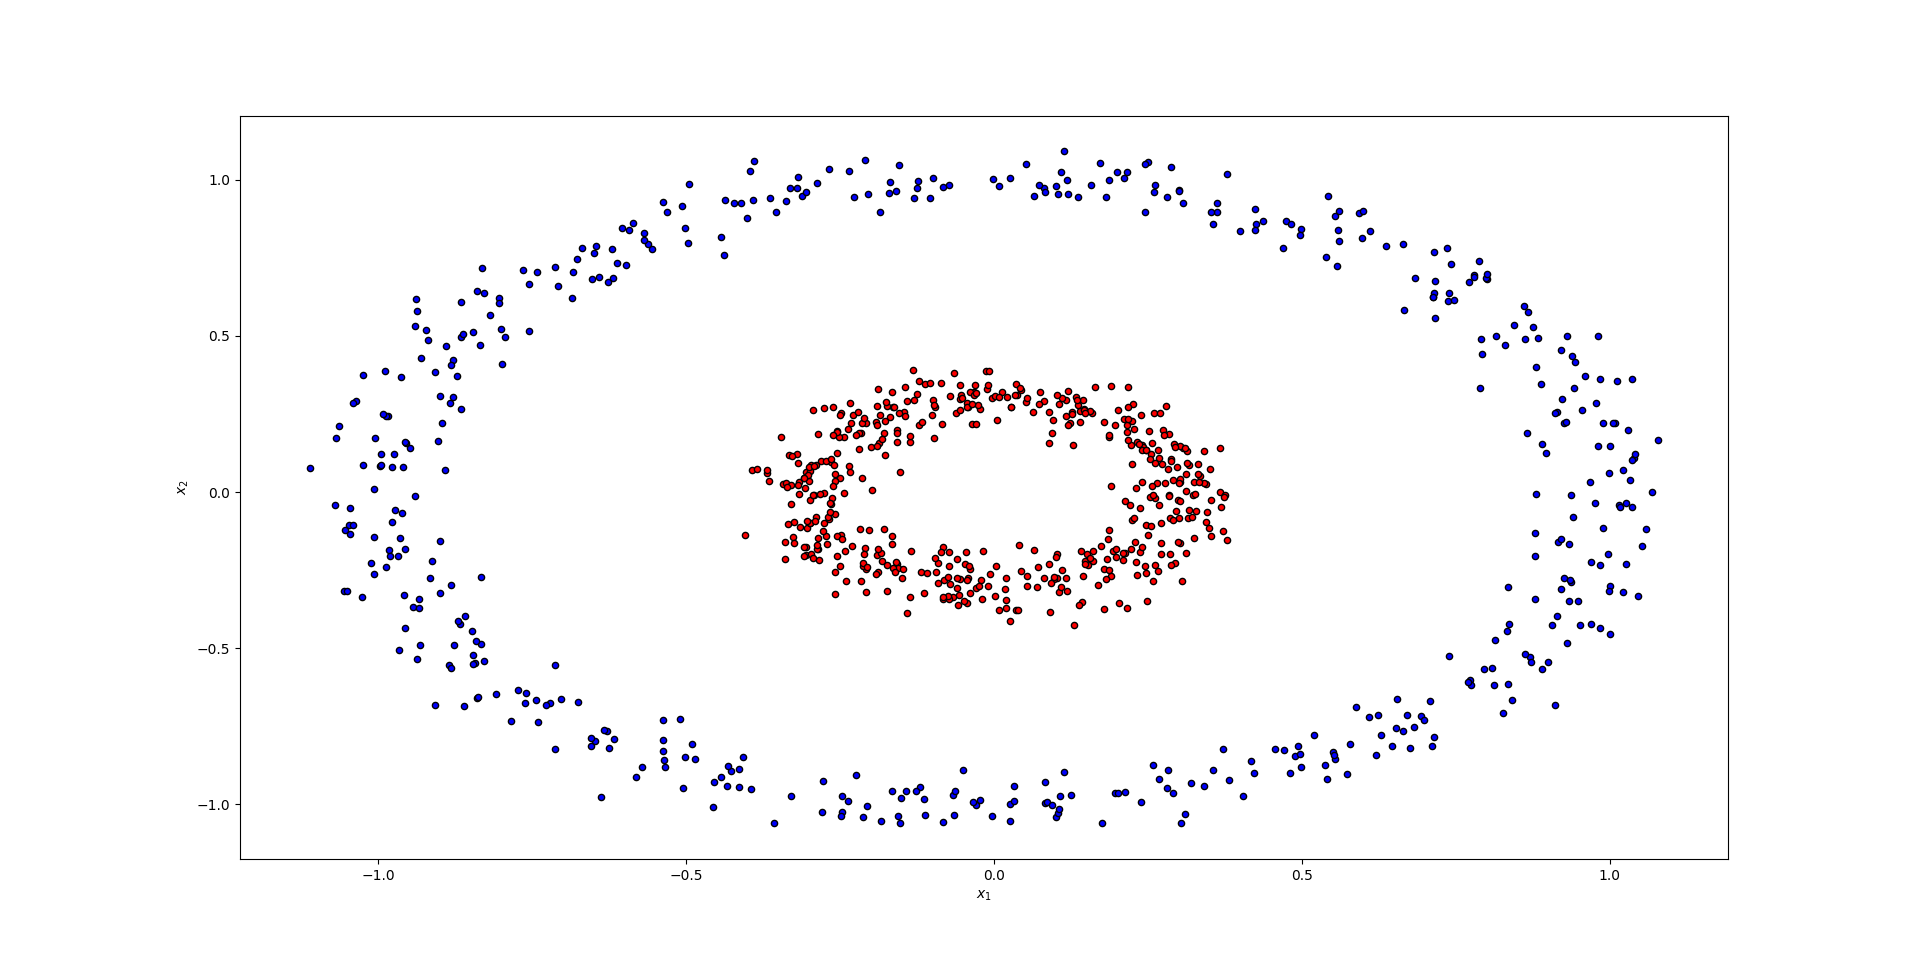
\includegraphics[width=.7\textwidth]{images/samples/circles}
				\caption{\label{fig::circles} Exemple de problème de classification non supervisée: Pas de classes mais une structure se dégage.}
			\end{center}
		\end{figure}
		\begin{itemize}
			\item[--]<1-> On observe que les instances ${(X^i)}_{i=1,\dots,n}$ sans les classes $\longrightarrow$ Classification non supervisée,
			\item[--]<2-> On observe des instances et leurs classes respectives ${\Big((X^i, Y^i)\Big)}_{i=1,\dots,n}$ $\longrightarrow$ Classification supervisée.
		\end{itemize}
	\end{frame}

	\begin{frame}{Discriminatif vs Génératif}
		Les échantillons réalise une loi de distribution inconnues $\mathbb{P}(X^i=x,Y^i=y)=p(x,y)$ et sont indépendents entre eux. La prédiction dépend de notre connaissance préalable:
		\begin{itemize}
			\item[--]<1-> On sait modéliser la distribution des classes et la réalisation des instances selon cette classe $p(x,y) = p(y).p(x\vert y)$ $\longrightarrow$ méthode générative,
			\begin{itemize}
				\item[--]<2-> Exemple: On suppose que la répartition des sexes est équilibrée dans le monde et que la répartition des mesures --- poids et taille --- suivent des lois gaussiennes (c.f Figure~\ref{fig::sample_2d});
			\end{itemize}
			\item[--]<3-> On n'a aucune connaissance \textit{a priori}. On cherche à apprendre un modèle de $ p(y \vert x) = \frac{p(x,y)}{p(x)}$ $\longrightarrow$ méthode discriminative,
			\begin{itemize}
				\item[--]<4-> Exemple: On apprend un modèle d'arbres aléatoires.
			\end{itemize}
		\end{itemize}
	\end{frame}

	\begin{frame}{Pourquoi classifier?}
		\begin{figure}[H]
			\ffigbox[\FBwidth]
			{
				\begin{subfloatrow}[2]
					\ffigbox[\FBwidth]
					{
						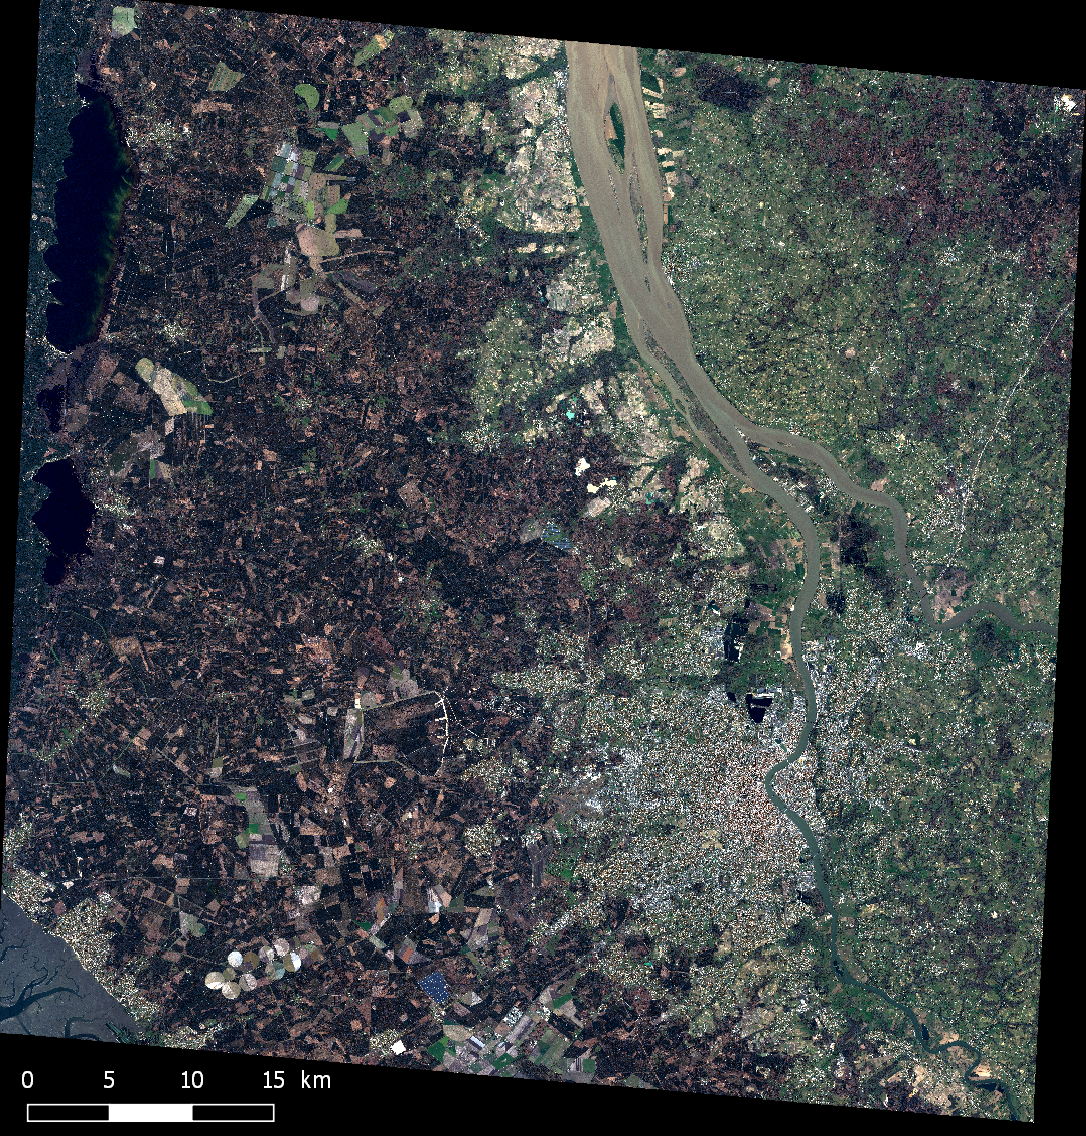
\includegraphics[width=.45\textwidth]{images/samples/gironde}
					}
					{
						\caption{Image de la Gironde prise par SPOT en 2016: Résolution $1.5m$, $4$ canaux: \{{\color{purple!20}Infrarouge}, {\color{red}Rouge}, {\color{green}Vert}, {\color{blue}Bleu}\}.}\label{fig::gir}
					}
					\ffigbox[\FBwidth]
					{
						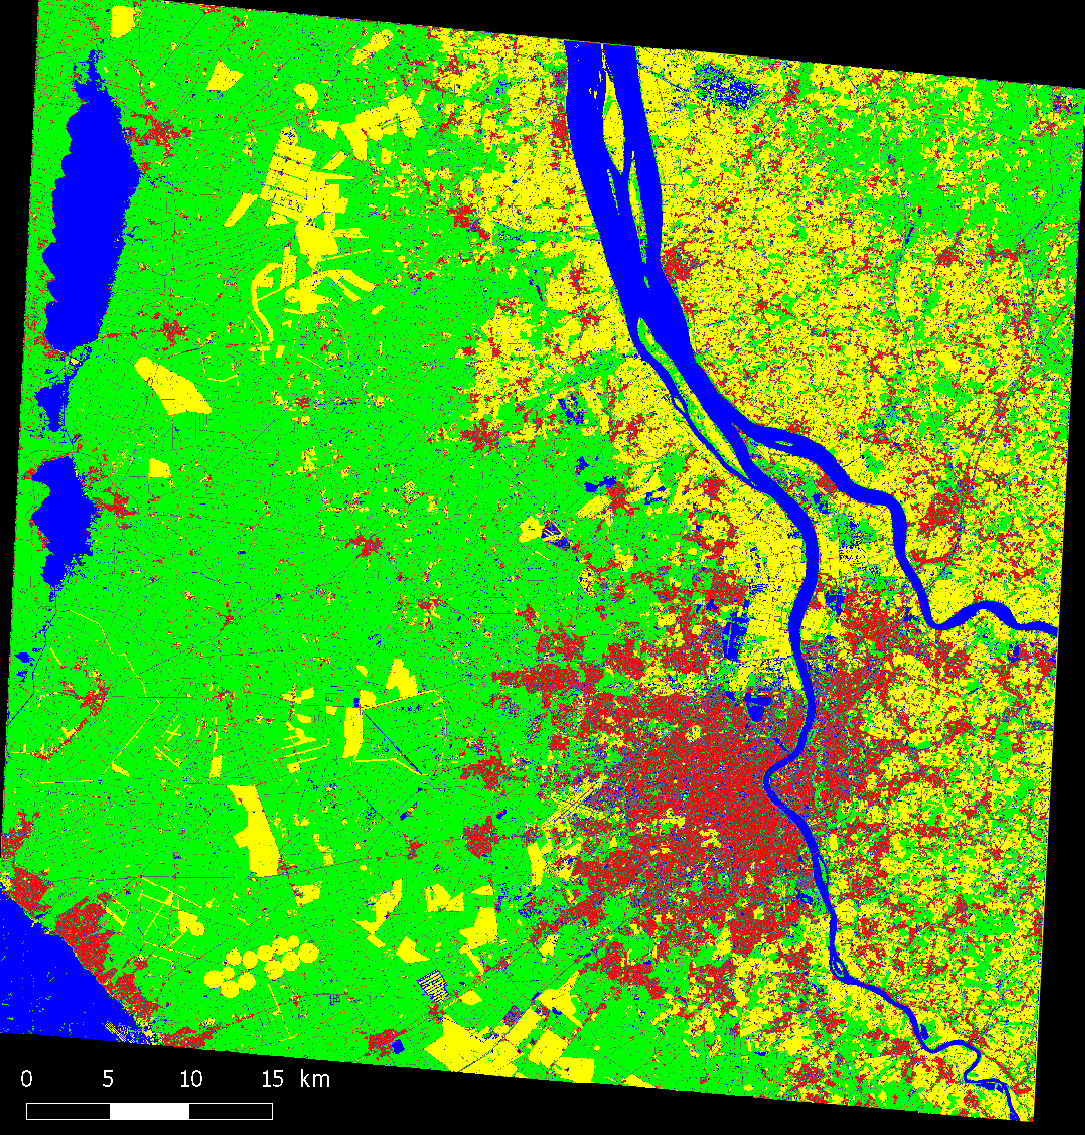
\includegraphics[width=.45\textwidth]{images/samples/gironde_classif}
					}
					{
						\caption{Occupation des sols extraite de l'image: {\color{red}$\blacksquare$} Bâti, {\color{green}$\blacksquare$} Forêt, {\color{yellow}$\blacksquare$} Culture, {\color{gray}$\blacksquare$} Routes, {\color{blue}$\blacksquare$} Eau.}\label{fig::gir_ocd}
					}
				\end{subfloatrow}
			}
			{
				\caption{\label{fig::ocs} Classification appliquée pour l'Occupation des sols~\cite{postadjian2017investigating}.}
			}
		\end{figure}
	\end{frame}

	\begin{frame}{Pourquoi classifier?}
		\begin{figure}[H]
			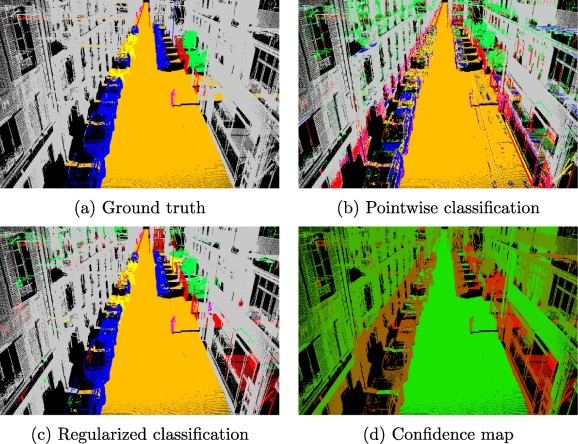
\includegraphics[width=.7\textwidth]{images/samples/pc_classification}
			\caption{\label{fig::pc_classif}Exemple de classification de nuage de point\cite{LANDRIEU2017102}.}
		\end{figure}
	\end{frame}

	\section[SVM]{SVM}
	\begin{frame}{Curse of dimensionality}
		\begin{itemize}
			\item[--]<1-> Si on a $n$ points à séparer, sans un modèle de classification, il y a un nombre exponentiel de séparations $\sum_{k=0,\dots,\lfloor \frac{n}{2} \rfloor} \begin{pmatrix}
			n\\
			k
			\end{pmatrix} = 2^{n-1}$ possibles $\longrightarrow$ C'est incalculable.
			\item[--]<2-> Il faut donc un modèle de séparation qui permettra de chercher efficacement une bonne solution: Forêts Aléatoires, \textbf{SVM}, Réseaux de Neurones \dots
		\end{itemize}
	\end{frame}
	\subsection[linear]{Séparateur linéaire}
	\begin{frame}{Mais c'est quoi donc ce SVM?}
		\begin{itemize}
			\item[--] SVM\@: Support Vector Machines;
			\item[--] C'est quoi un vecteur support?
		\end{itemize}
	\end{frame}

	\begin{frame}{Séparateur}
		On se place dans le cas de classification binaire:
		$$ X^i \in \mathbb{R}^d , \quad \forall i=1,\dots,n$$
		$$ Y^i \in \{-1, +1\} , \quad \forall i=1,\dots,n$$
		\begin{itemize}
			\item[--]On cherche une fonction qui estime la probabilité:
			$$ \eta(x) = p(y = 1 \vert x) = 1 - p(y = -1 \vert x)$$
			\item[--] On peut y arriver en modélisant:
			\begin{align*}
				f: x \mapsto \mathbb{E}_Y(Y \vert X=x) &= \sum_{y=-1, +1} Y.p(Y\vert X=x)\\
				&= (+1) \times p(y = 1\vert x) + (-1) \times p(y = -1\vert x)
			\end{align*}

			à partir duquel on déduit la fonction de décision:
			\begin{align*}
				D: \mathbb{R}^d &\rightarrow \{-1, +1\} \\
				x &\mapsto D(x) = sign(f(x))
			\end{align*}
			\item[--] Le séparateur est la courbe qui vérifie:
			\begin{align*}
				\mathscr{S} &\triangleq \{X \in \mathbb{R}^d: f(X) = 0\} \\
							&= \{X \in \mathbb{R}^d: p(1\vert x) = p(-1\vert x)\}
			\end{align*}
		\end{itemize}
	\end{frame}

	\begin{frame}{Séparateur}
		\begin{figure}[H]
			\ffigbox[\FBwidth]
			{
				\begin{subfloatrow}[2]
					\ffigbox[\FBwidth]
					{
						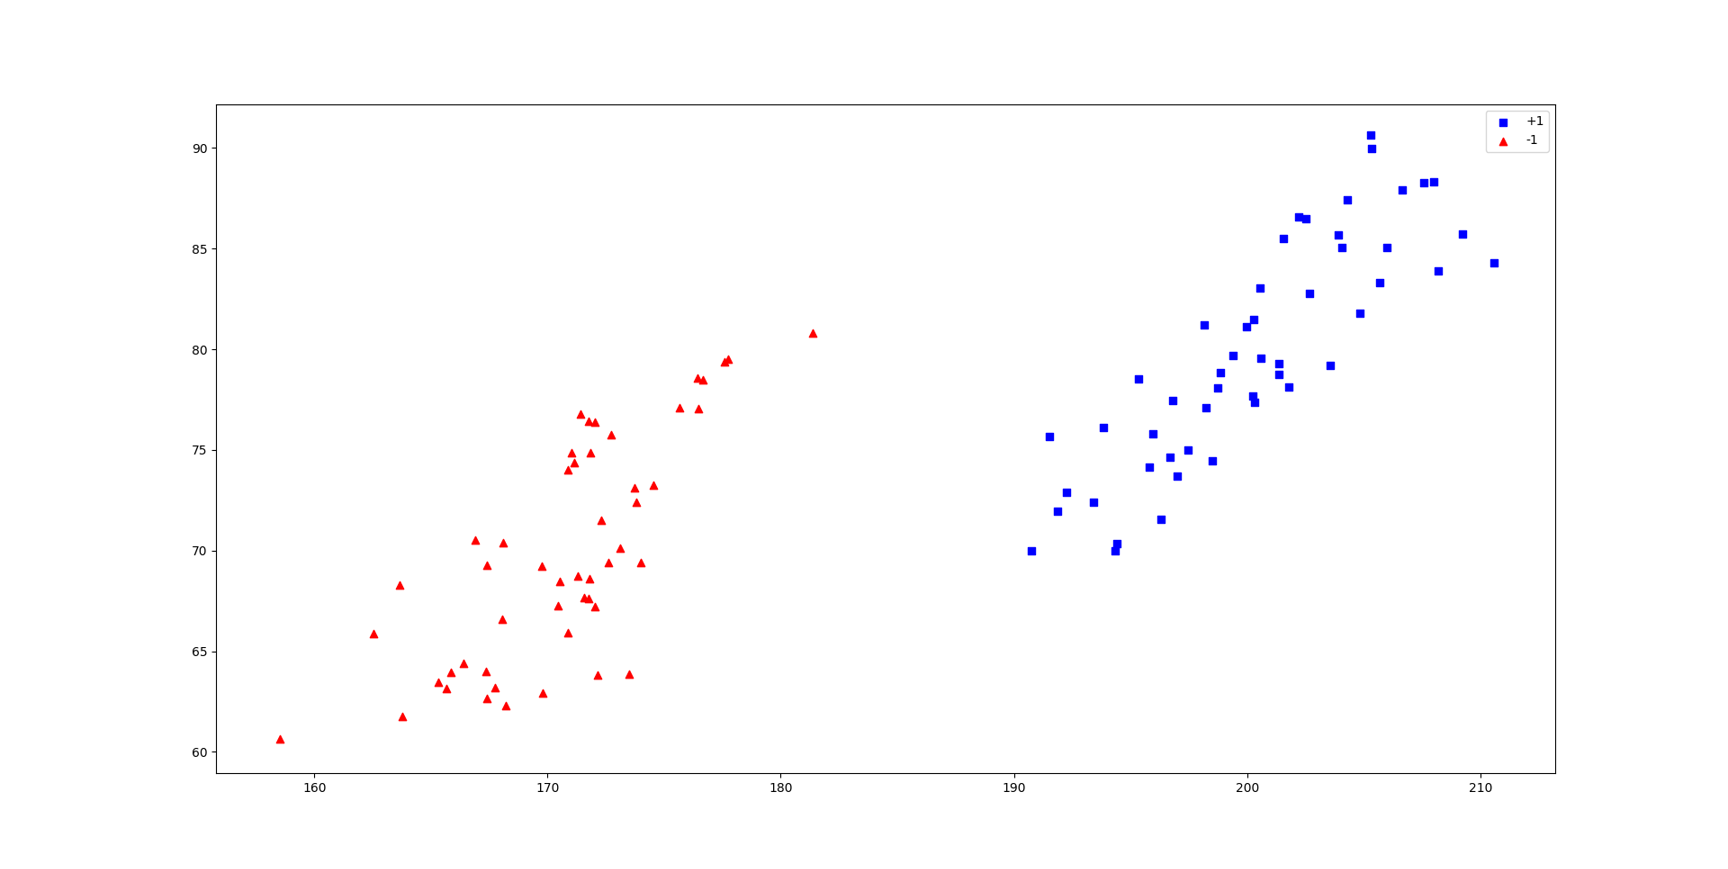
\includegraphics[width=.45\textwidth]{images/samples/sample_svm}
					}
					{
						\caption{Echantillons à séparer.}\label{fig::sample_sep}
					}
					\ffigbox[\FBwidth]
					{
						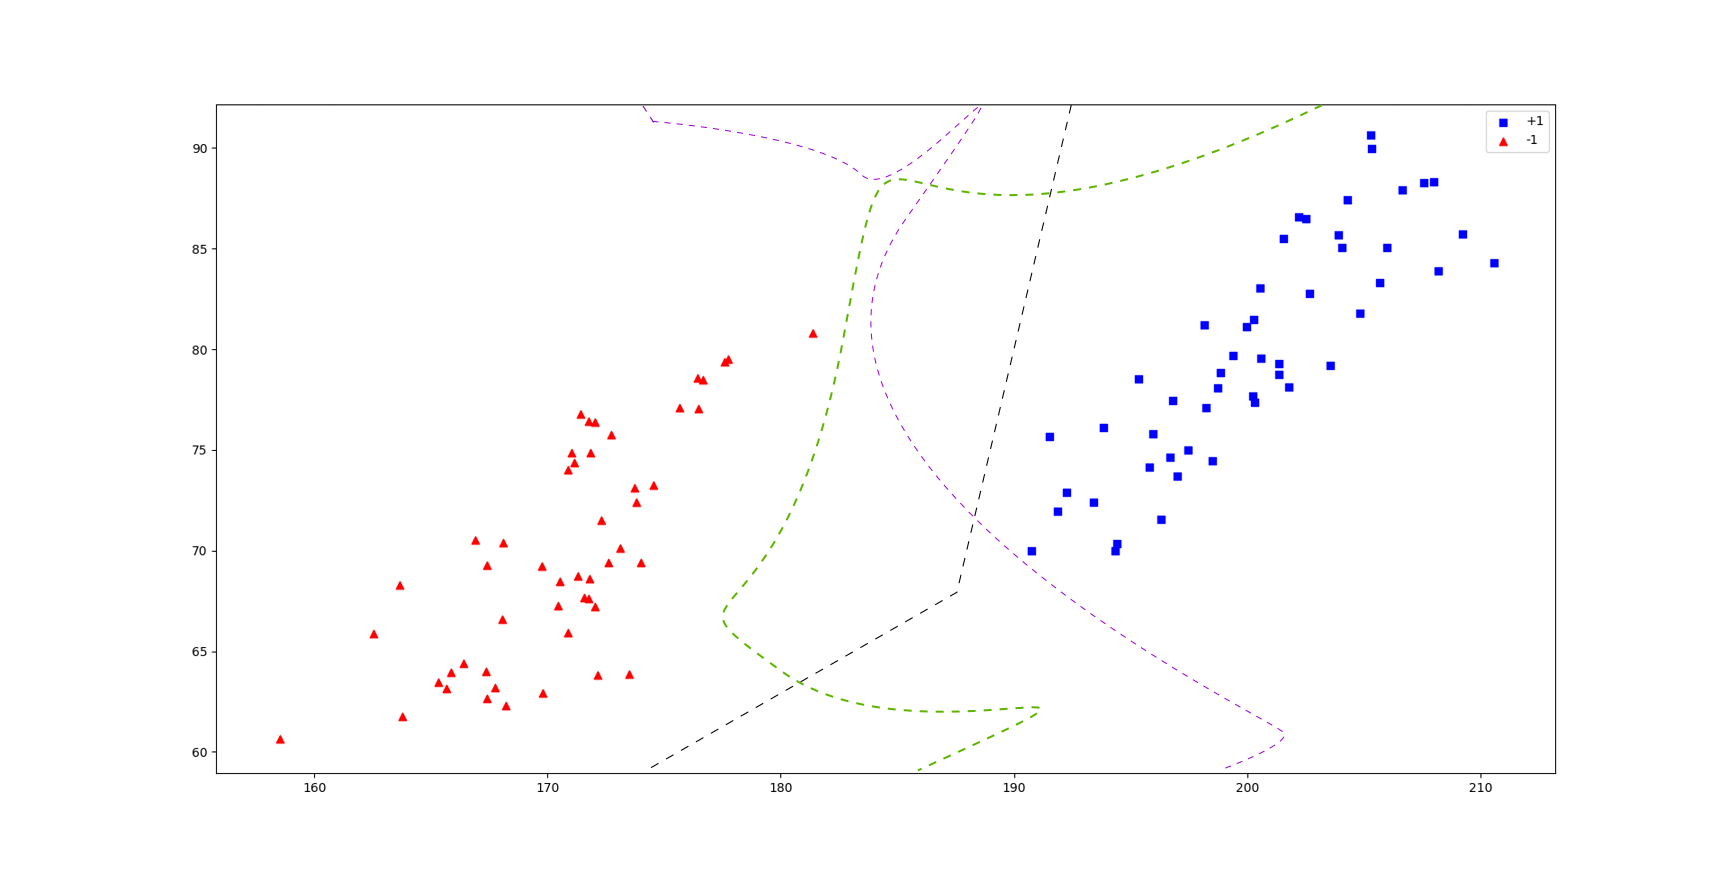
\includegraphics[width=.45\textwidth]{images/samples/separators}
					}
					{
						\caption{Séparateurs possibles.}\label{fig::sep_ex}
					}
				\end{subfloatrow}
			}
			{
				\caption{\label{fig::separators} Séparation de données.}
			}
		\end{figure}
	\end{frame}

	\begin{frame}{Choix du séparateur}
		\begin{itemize}
			\item[--] Il y a une infinité de modèle de $f(X)$ possible.
			\item[--] Le choix le plus naïf serait de donner, pour chaque instance d'entraînement, la valeur qui lui est associé, en ignorant le reste des points possibles:
			\begin{equation*}
				f = \sum_{i=1,\dots,n} Y^i . \delta_{X^i}
			\end{equation*}
			Cependant, ce classifieur n'a aucun pourvoir de généralisation. En effet:
			\begin{gather*}
				\widetilde{x} \leftarrow \sum_{i=1,\dots,n} X^i \notin \{X^i, \forall i=1,\dots,n\} \\
				\Rightarrow f(\widetilde{x}) = 0
			\end{gather*}
			\item[--] On s'intéresse, dans le cadre du cours, aux séparateurs linéaires:
			\begin{align*}
				f_{\textbf{w}, b}: \mathbb{R}^d &\rightarrow \{-1, 0, +1\} \\
				\textbf{x} &\mapsto f_{\textbf{w}, b}(\textbf{x}) = \textbf{w}.\textbf{x} + b
			\end{align*}
		\end{itemize}
	\end{frame}

	\begin{frame}{Séparateur linéaire}
		\begin{figure}[H]
			\ffigbox[\FBwidth]
			{
				\begin{subfloatrow}[2]
					\ffigbox[\FBwidth]
					{
						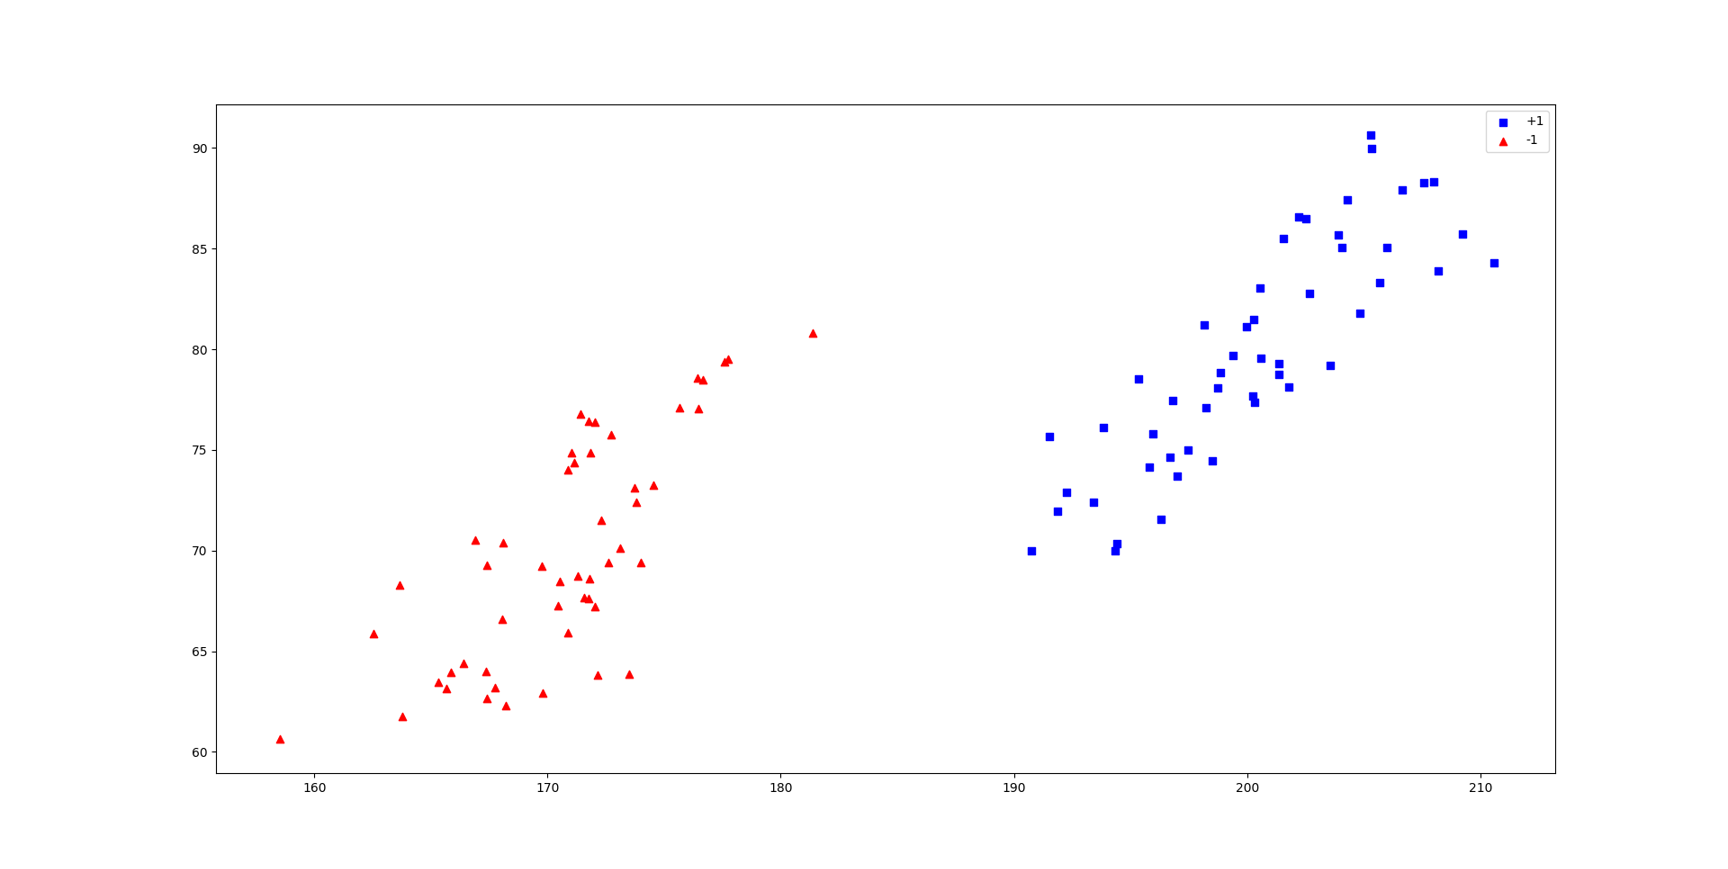
\includegraphics[width=.45\textwidth]{images/samples/sample_svm}
					}
					{
						\caption{Echantillons à séparer.}\label{fig::sample_sep2}
					}
					\ffigbox[\FBwidth]
					{
						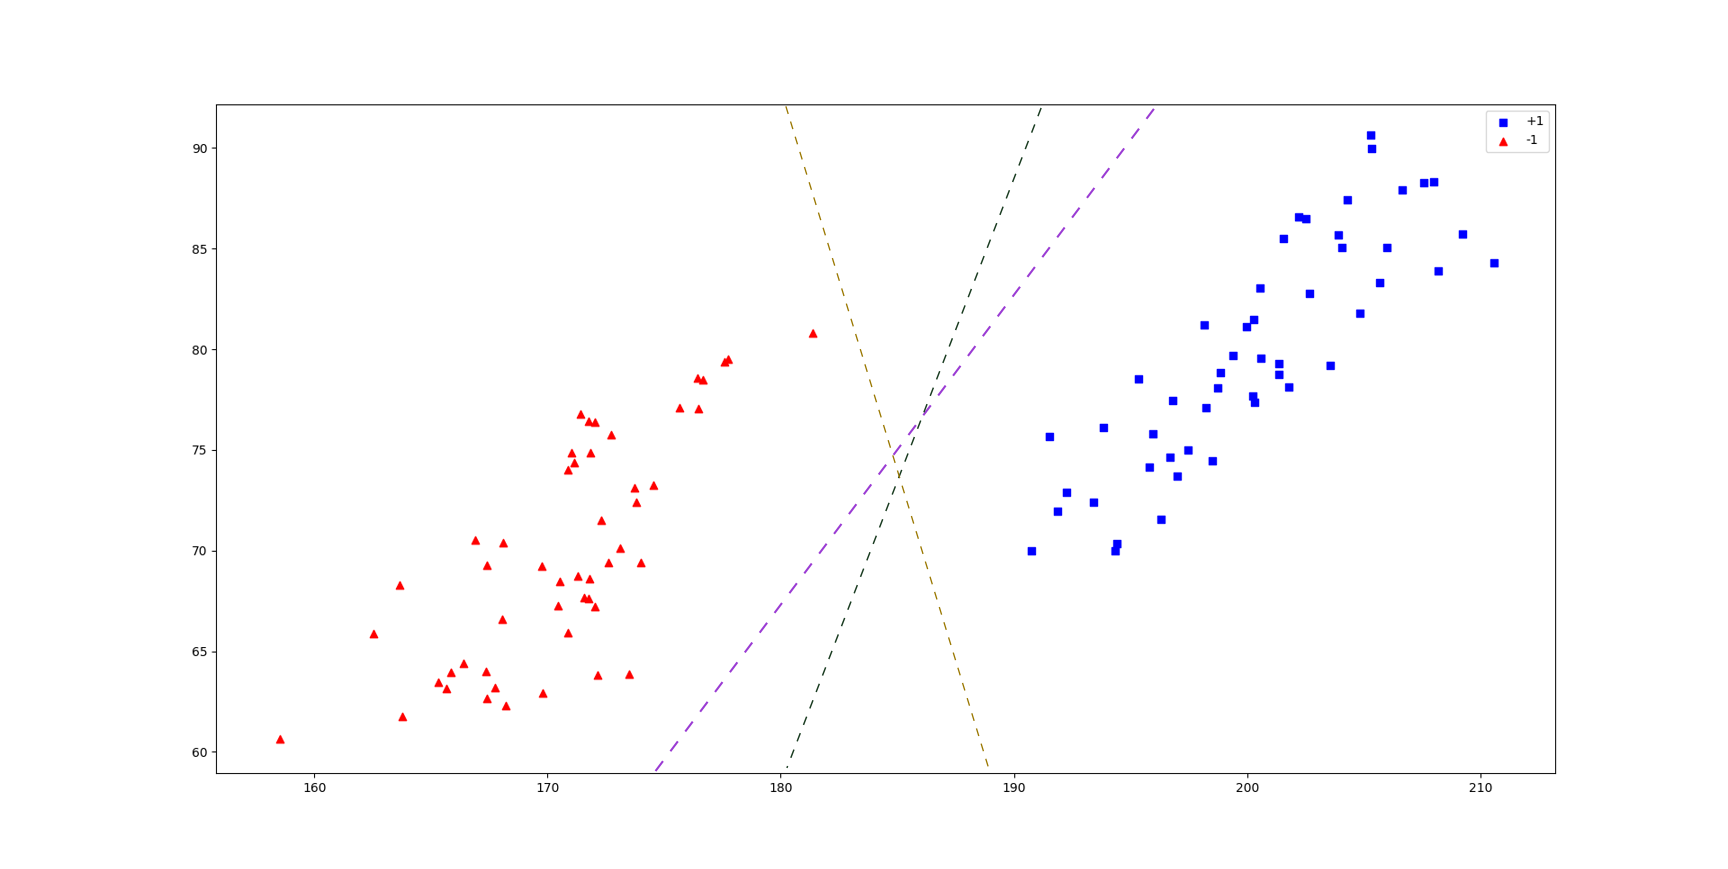
\includegraphics[width=.45\textwidth]{images/samples/linear_separation}
					}
					{
						\caption{Exemples de séparateurs linéaires possibles.}\label{fig::lin_sep}
					}
				\end{subfloatrow}
			}
			{
				\caption{\label{fig::lin_separators} Séparation linéaire de données.}
			}
		\end{figure}
	\end{frame}

	\subsection[linear]{SVM linéaire}
	\begin{frame}{Mais c'est quoi donc ce SVM?}
		\begin{itemize}
			\item[--] SVM\@: Support Vector Machines.
			\item[--] C'est quoi donc un vecteur support?
			\item[--] Quelle est la relation avec les séparateurs linéaires?
		\end{itemize}
	\end{frame}

	\begin{frame}{SVM\@: maximiser la marge.}
		\begin{figure}[H]
			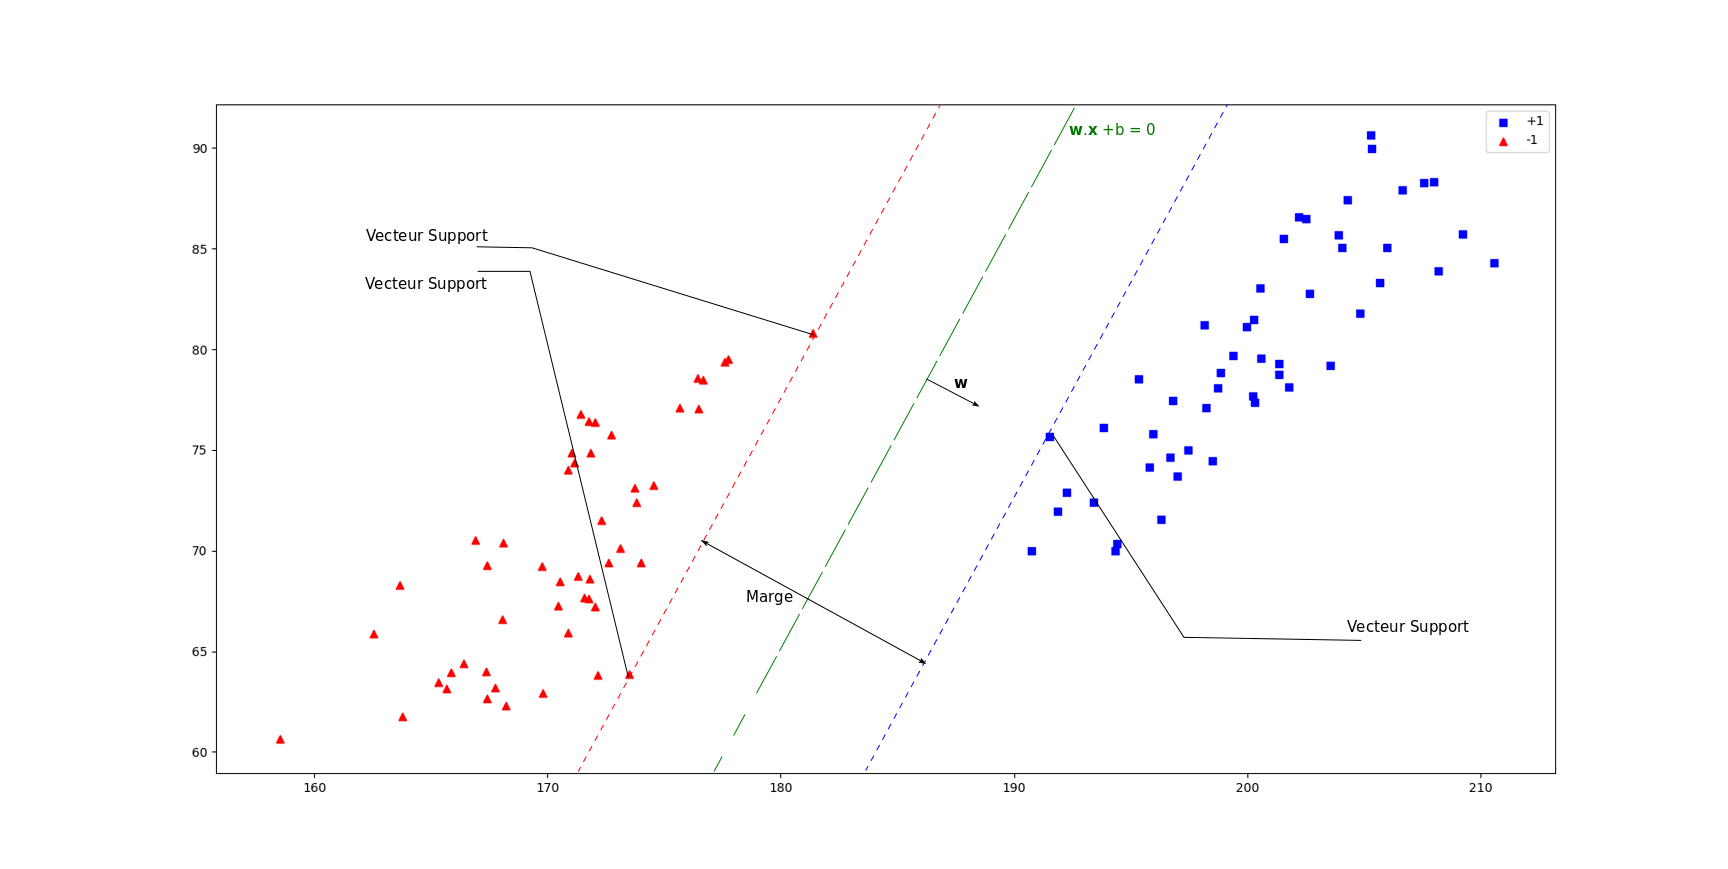
\includegraphics[width=\textwidth]{images/samples/svm}
			\caption{\label{fig::svm} Le séparateur linéaire SVM.}
		\end{figure}
	\end{frame}

	\begin{frame}{SVM\@: maximiser la marge.}
		\begin{itemize}
			\item[--] Le but du SVM est de maximiser la marge~\cite{vapnik1998statistical}.
			\item[--] On remarque que:
			\begin{gather*}
				\textbf{w} \in \{\omega \in \mathbb{R}^d : f_{\omega, b} = \mathbb{0}\} \\
				\Rightarrow
				\lambda . \textbf{w} \in \{\omega \in \mathbb{R}^d : f_{\omega, b} = \mathbb{0}\}\quad, \forall \lambda \in \mathbb{R}\setminus\{0\}
			\end{gather*}
			\item[--] Il y a donc une infinité de solutions possibles. On prend donc la solution $\textbf{w}$ qui permet d'avoir:
			\begin{align}
				\textbf{w}.\textbf{x}_{\color{blue}+} + b &= {\color{blue}+}1 \\
				\textbf{w}.\textbf{x}_{\color{red}-} + b &= {\color{red}-}1
			\end{align}
			où:
			\begin{itemize}
				\item[{\color{blue}+}] $\textbf{x}_{\color{blue}+}$ correspond aux supports vecteurs positifs (i.e. $Y={\color{blue}+}1$).
				\item[{\color{red}---}] $\textbf{x}_{\color{red}-}$ correspond aux supports vecteurs négatifs (i.e. $Y={\color{red}-}1$).
			\end{itemize}
		\end{itemize}
	\end{frame}

	\begin{frame}{SVM\@: maximiser la marge.}
		\begin{figure}[H]
			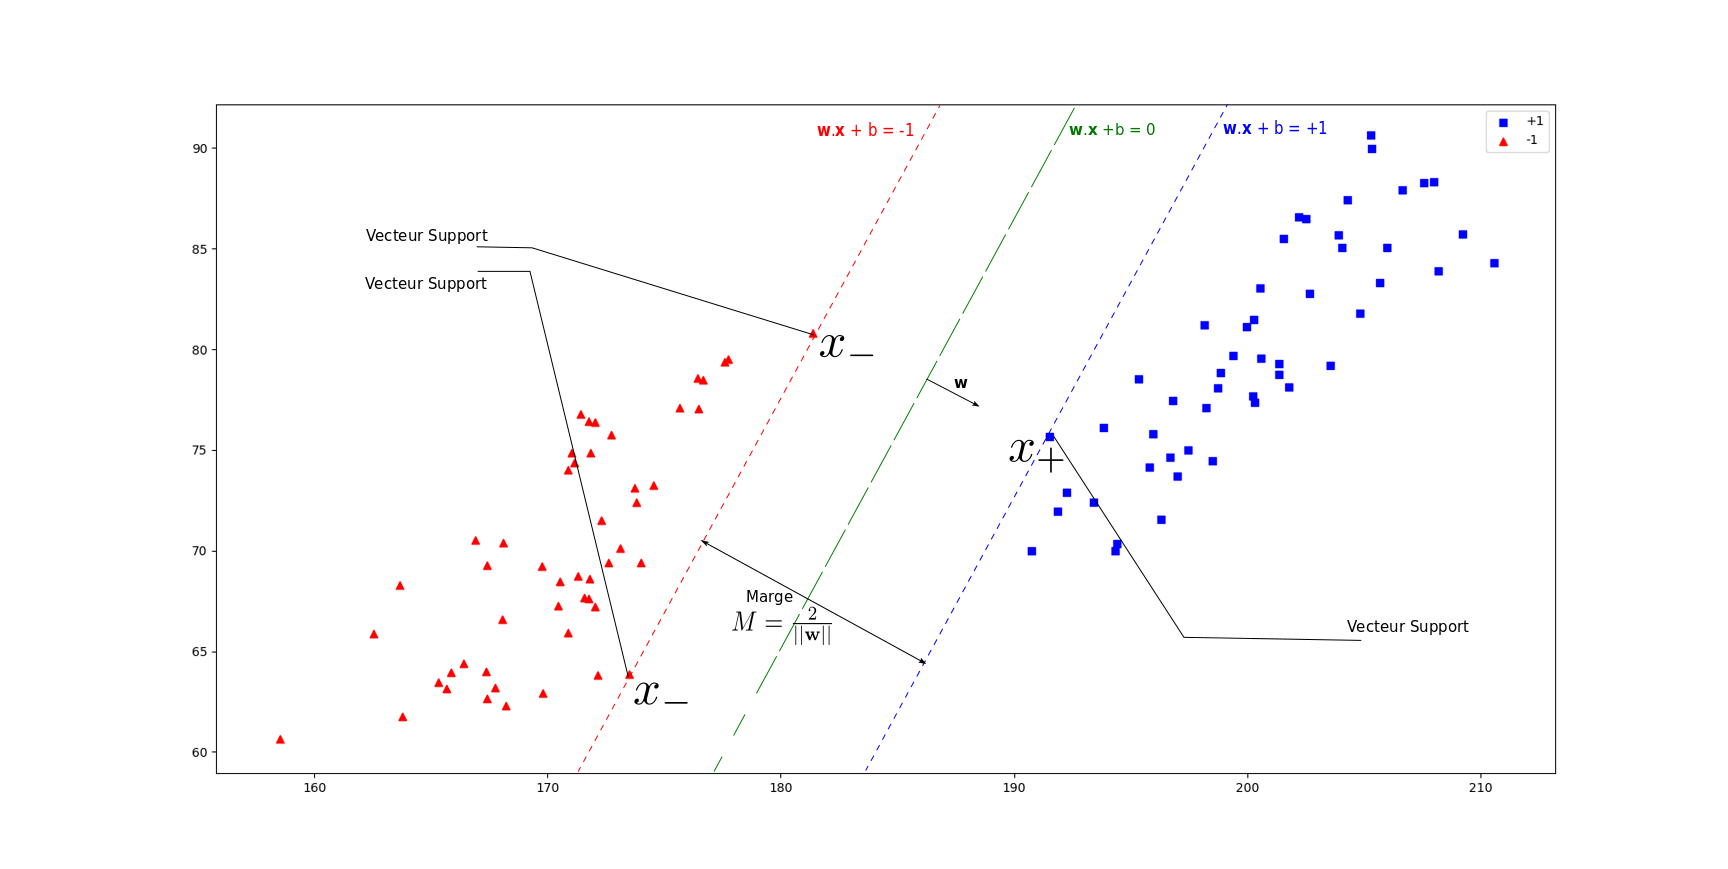
\includegraphics[width=\textwidth]{images/samples/svm_margin}
			\caption{\label{fig::margin} Le séparateur linéaire SVM.}
		\end{figure}
	\end{frame}

	\begin{frame}{SVM\@: optimisation.}
		\begin{itemize}
			\item[--] On cherche à maximiser la marge:
			\begin{align}
				M &= \frac{\textbf{w}.(\textbf{x}_+ - \textbf{x}_-)}{\vert\vert \textbf{w} \vert\vert} \\
				  &= \frac{2}{\vert\vert \textbf{w} \vert\vert}
			\end{align}
			\item[--] Le problème est reformuler donc comme suit:
			\begin{equation}
				\begin{aligned}
				& \max_{\textbf{w}}
				& & \frac{2}{\vert\vert \textbf{w} \vert\vert} \\
				& \text{sous contrainte}
				& & \begin{cases}
					\textbf{w}.\textbf{X}^i + b \leq -1 & Y^i = -1 \\
					\textbf{w}.\textbf{X}^i + b \geq 1 & Y^i = 1
				\end{cases} \; \forall i = 1, \dots, n.
				\end{aligned}
			\end{equation}
			\item[--] Ou encore:
			\begin{equation}
				\begin{aligned}
				& \min_{\textbf{w}}
				& & {\vert\vert \textbf{w} \vert\vert}^2 \\
				& \text{sous contrainte}
				& & Y^i.(\textbf{w}.\textbf{X}^i + b) \geq 1 \; \forall i = 1, \dots, n.
				\end{aligned}
			\end{equation}
		\end{itemize}
	\end{frame}

	\begin{frame}{Cas non séparable.}
		\begin{figure}[H]
			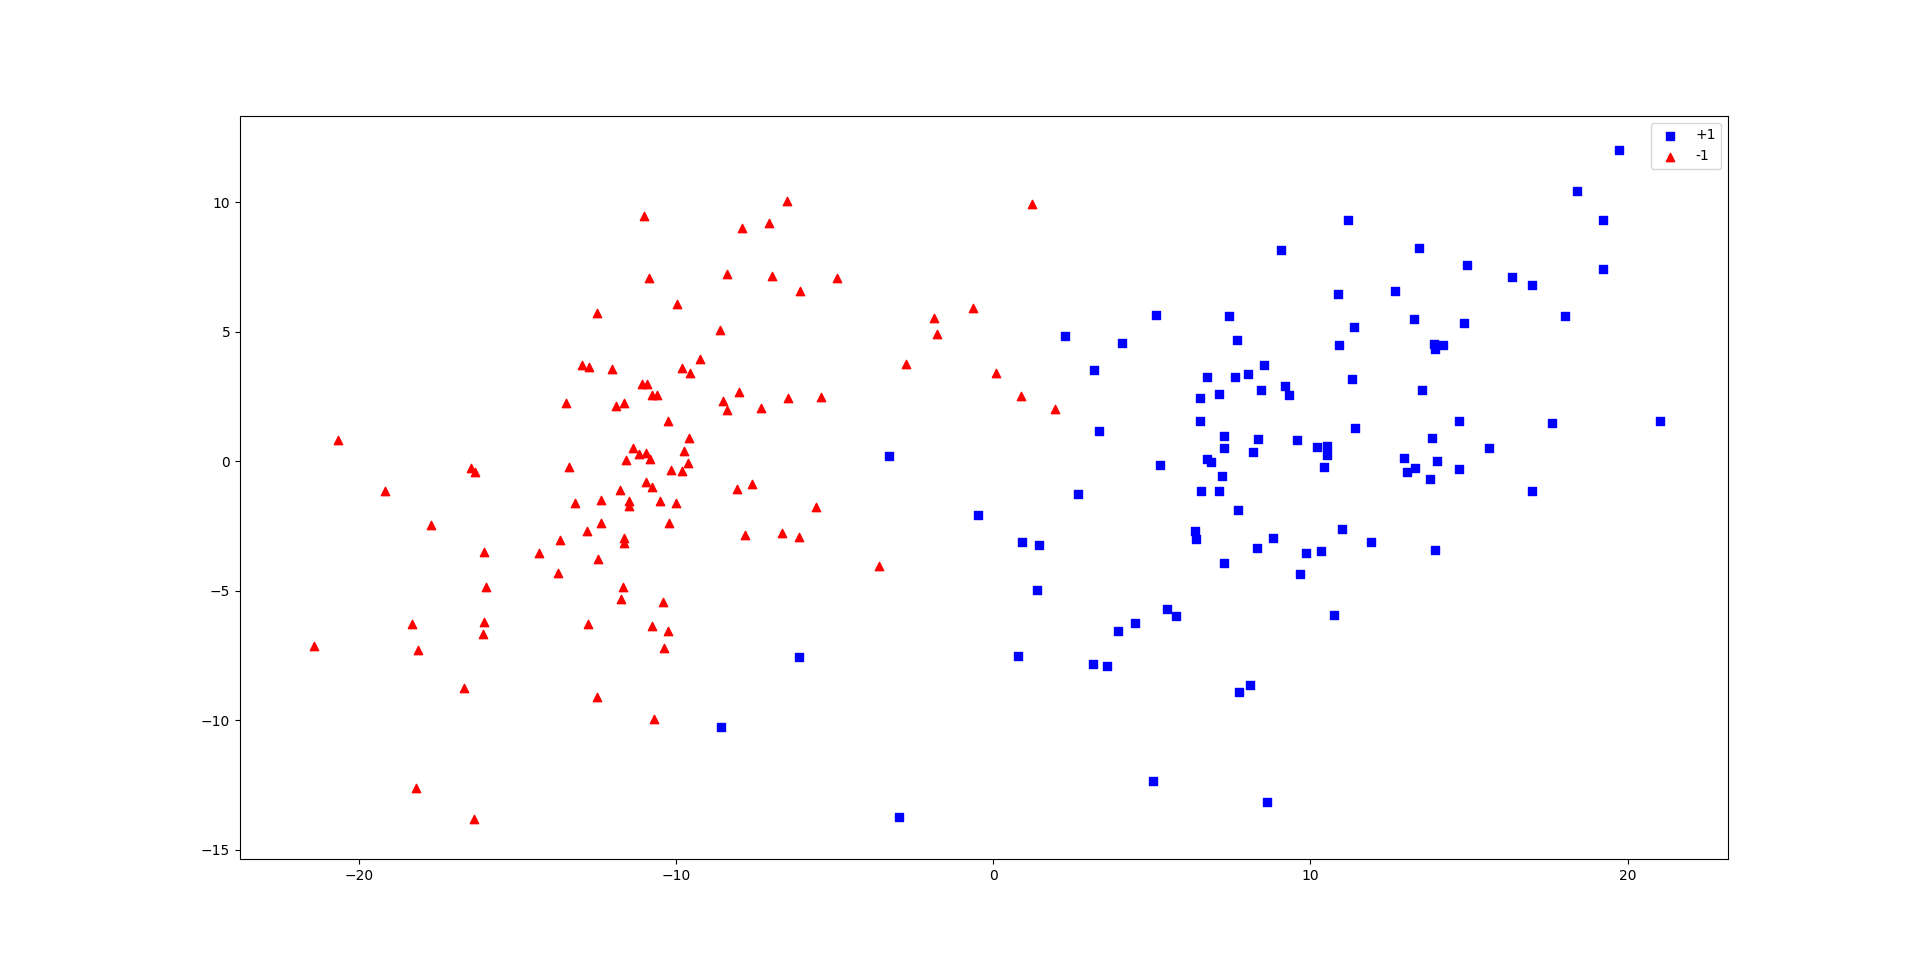
\includegraphics[width=\textwidth]{images/samples/non_separable}
			\caption{\label{fig::non_sep} Le séparateur linéaire SVM.}
		\end{figure}
	\end{frame}

	\begin{frame}{Cas non séparable.}
		\begin{figure}[H]
			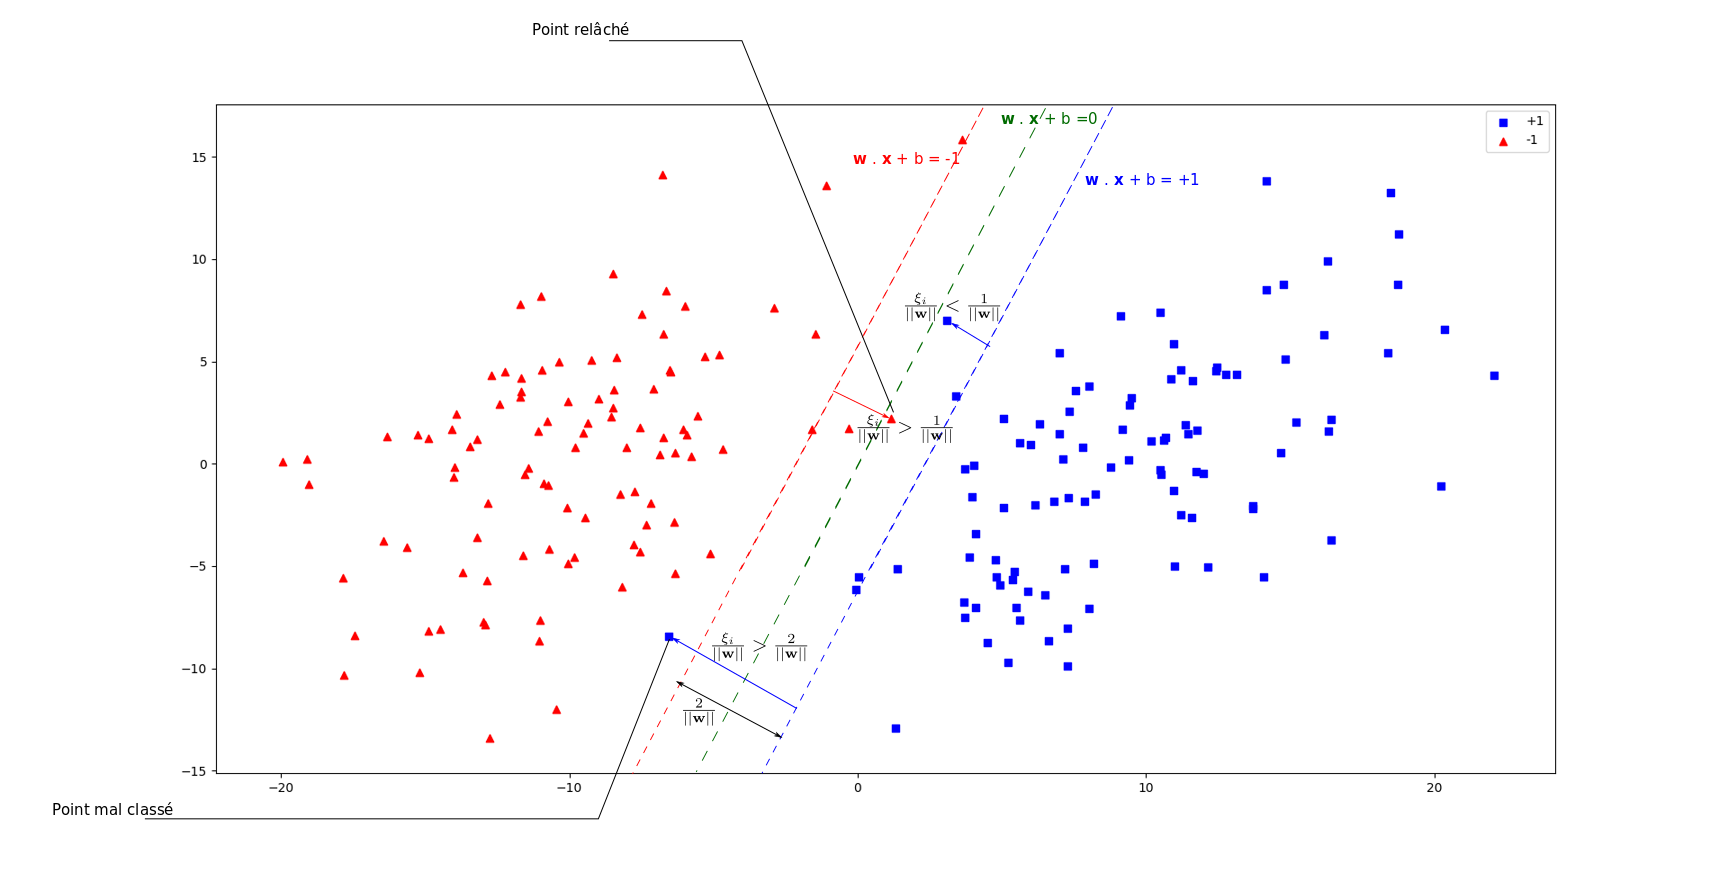
\includegraphics[width=\textwidth]{images/samples/stable_margin}
			\caption{\label{fig::stable_margin} La marge du séparateur linéaire SVM.}
		\end{figure}
	\end{frame}

	\begin{frame}{Cas non séparable.}
		\begin{itemize}
			\item[--] On lâche du ``mou'': On accepte des fois que
			$$\exists k \; Y^k.(\textbf{w}.\textbf{X}^k + b) < 1$$
			\item[--] On peut écrire ceci autrement:
			$$\forall i=1,\dots,n \quad \exists \xi_i \geq 0 \quad Y^i.(\textbf{w}.\textbf{X}^i + b) \geq 1 - \xi_i$$

			\item[--] Il y a donc quatres cas pour $ \xi_i $:
			\begin{itemize}
				\item[-] $\xi_i = 0 \Rightarrow$ Point bien classé;
				\item[-] $0 < \xi_i \leq 1 \Rightarrow$ Point situé dans la marge: bien classé mais moins sûr;
				\item[-] $1 < \xi_i \Rightarrow$ Point de l'autre côté de la ligne séparatrice mais dans la marge: donc mal classé et pas très sûr;
				\item[-] $2 < \xi_i \Rightarrow$ Point non séparable, il dépasse l'autre limite de marge: sûrement mal classé;
			\end{itemize}

			\item[--] Dans le cas ou le problème n'est pas séparable linéairement, on peut déduire que
			$\exists j, \quad 2 < \xi_j$

			\item[--] N'importe quel droite peut ainsi séparer les données. Les différents $\xi_i$ peuvent donc être très grand. Par conséquent, il faut les pénaliser au moment de l'optimisation. Le problème devient:
			\begin{equation}
				\begin{aligned}
				& \min_{\textbf{w}, \xi_1,\dots,\xi_n \in \mathbb{R}^+}
				& & {\vert\vert \textbf{w} \vert\vert}^2 + C.\sum_{i=1,\dots,n}\xi_i\\
				& \text{sous contrainte}
				& & Y^i.(\textbf{w}.\textbf{X}^i + b) \geq 1 - \xi_i , \forall i = 1, \dots, n.
				\end{aligned}
			\end{equation}
		\end{itemize}
	\end{frame}

	\begin{frame}{Cas de la constante de régularisation}
		\begin{itemize}
			\item[--] $C \ll 1 \Longrightarrow$ moins de pénalisation sur les variables de ressort $\Longrightarrow$ marge très grande, plus de généralisation;
			\item[--] $C \gg 1 \Longrightarrow$ plus de pénalisation sur les variables de ressort $\Longrightarrow$ marge serrée, moins de généralisation;
			\item[--] $C=\infty \Longrightarrow$ pénalisation complète sur les variables de ressort $\Longrightarrow$ marge dure: c'est la première version de SVM qu'on a vu.
		\end{itemize}
	\end{frame}
	\begin{frame}{Optimization Quadratique! Peut-on faire mieux?}
		\begin{itemize}
			\item[--] Problème primal (Quadratique):
			\begin{equation}
				\begin{aligned}
				& \min_{\textbf{w}, \xi_1,\dots,\xi_n \in \mathbb{R}^+}
				& & {\vert\vert \textbf{w} \vert\vert}^2 + C.\sum_{i=1,\dots,n}\xi_i \\
				& \text{sous contrainte}
				& & Y^i.(\textbf{w}.\textbf{X}^i + b) \geq 1 - \xi_i , \forall i = 1, \dots, n.
				\end{aligned}
			\end{equation}
			\item[--] Problème dual:
			\begin{equation}
				\begin{aligned}
				& \max_{0 \leq \alpha_i \leq C ,\forall i=1,\dots,n}
				& & \sum_{i=1,\dots,n} \alpha_i - \frac{1}{2}.\sum_{l,p=1,\dots,n}\alpha_l.\alpha_p.Y^l.Y^p.(X^l.X^p)\\
				& \text{sous contrainte}
				& & \sum_{i=1,\dots,n}Y^i.\alpha_i=0
				\end{aligned}
			\end{equation}
            \item[--] Ce dernier est un problème d'optimisation \textit{linéaire} qu'on sait résoudre plus facilement.
		\end{itemize}
	\end{frame}
    \begin{frame}{Algorithmes en Pratiques}

		On admet que la résolution d'un problème est équivalente à la résolution de l'autre.
		\begin{itemize}
			\item[--] Problème Primal: Stochstic Gradient Descent~\cite{bottou2010} (SGD).
            \item[--] Problème Dual: Sequential minimal Optimization (SMO)~\cite{platt1998sequential} et dérivées.
		\end{itemize}
	\end{frame}
	\subsection[kernel]{Kernel SVM}

	\begin{frame}{Changement d'espace}
		\begin{figure}[H]
			\begin{center}
				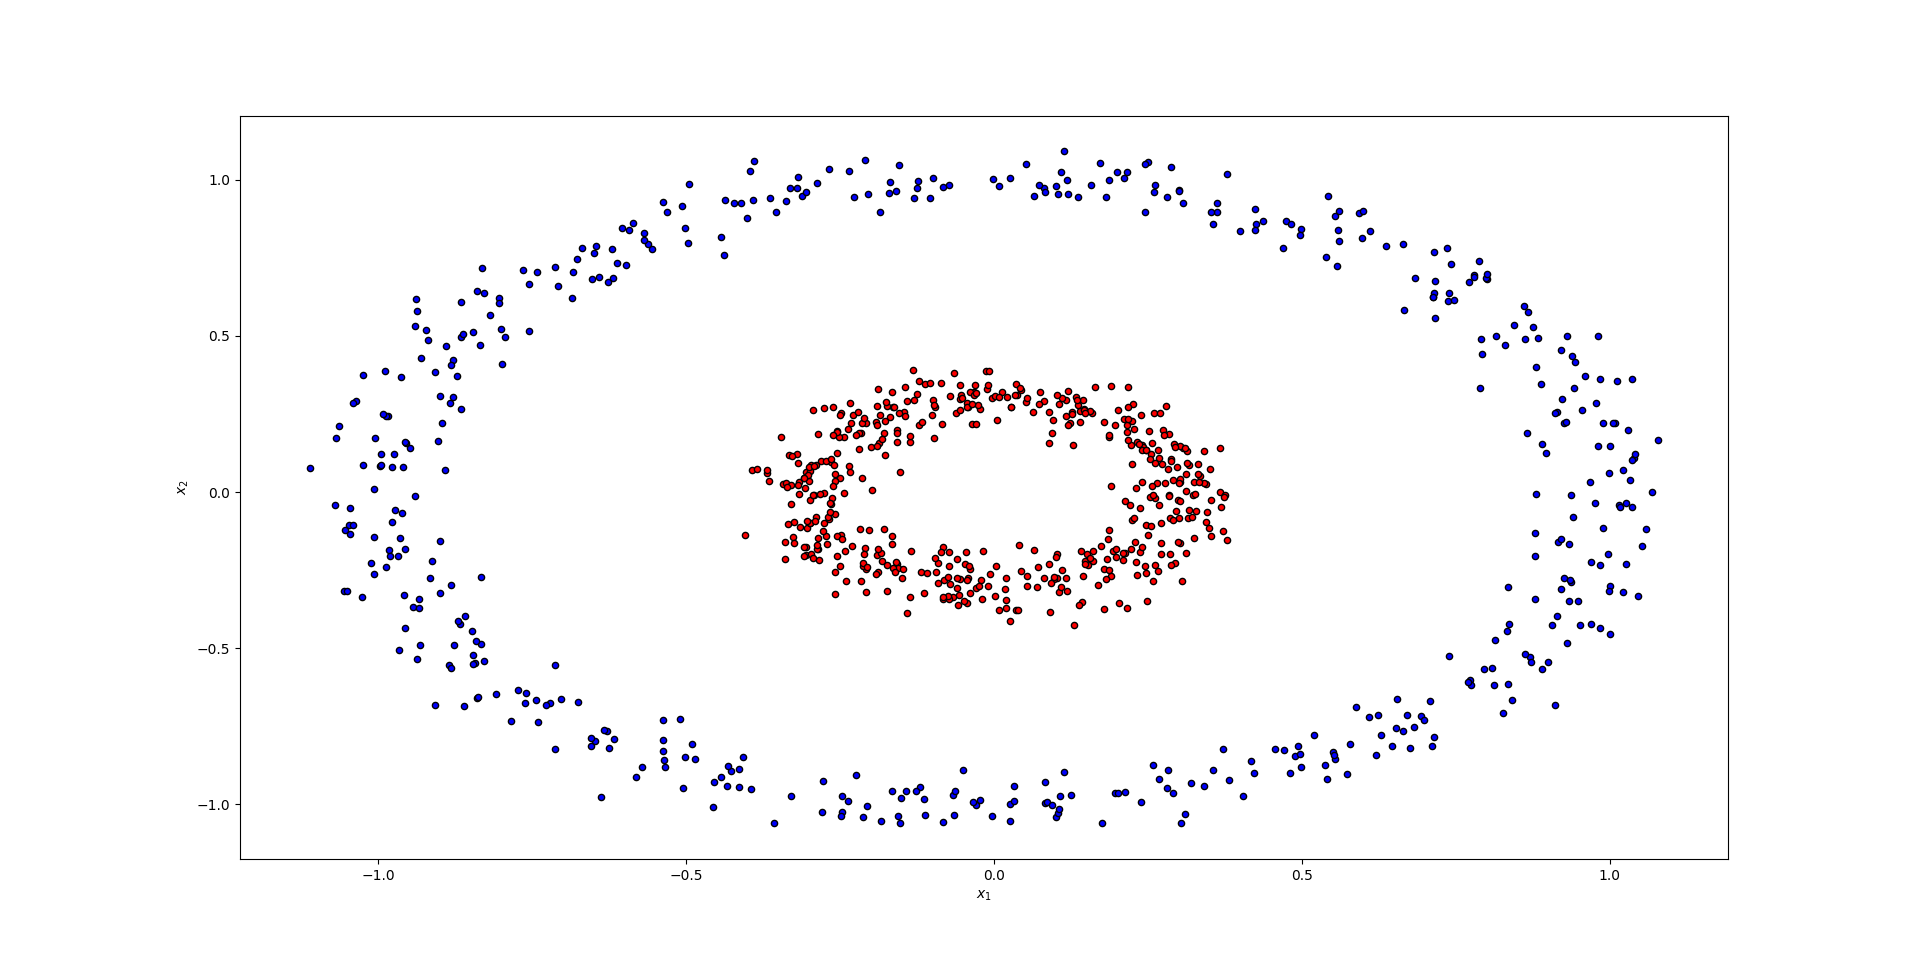
\includegraphics[width=.7\textwidth]{images/samples/circles}
				\caption{\label{fig::circles_3} Quelle transformation à appliquer pour obtenir des instances séparables linéairement.}
			\end{center}
		\end{figure}
	\end{frame}
	\begin{frame}{Changement d'espace}
		\begin{itemize}
			\item[--] Trouver la transformation $\Phi$:
			\begin{figure}[H]
				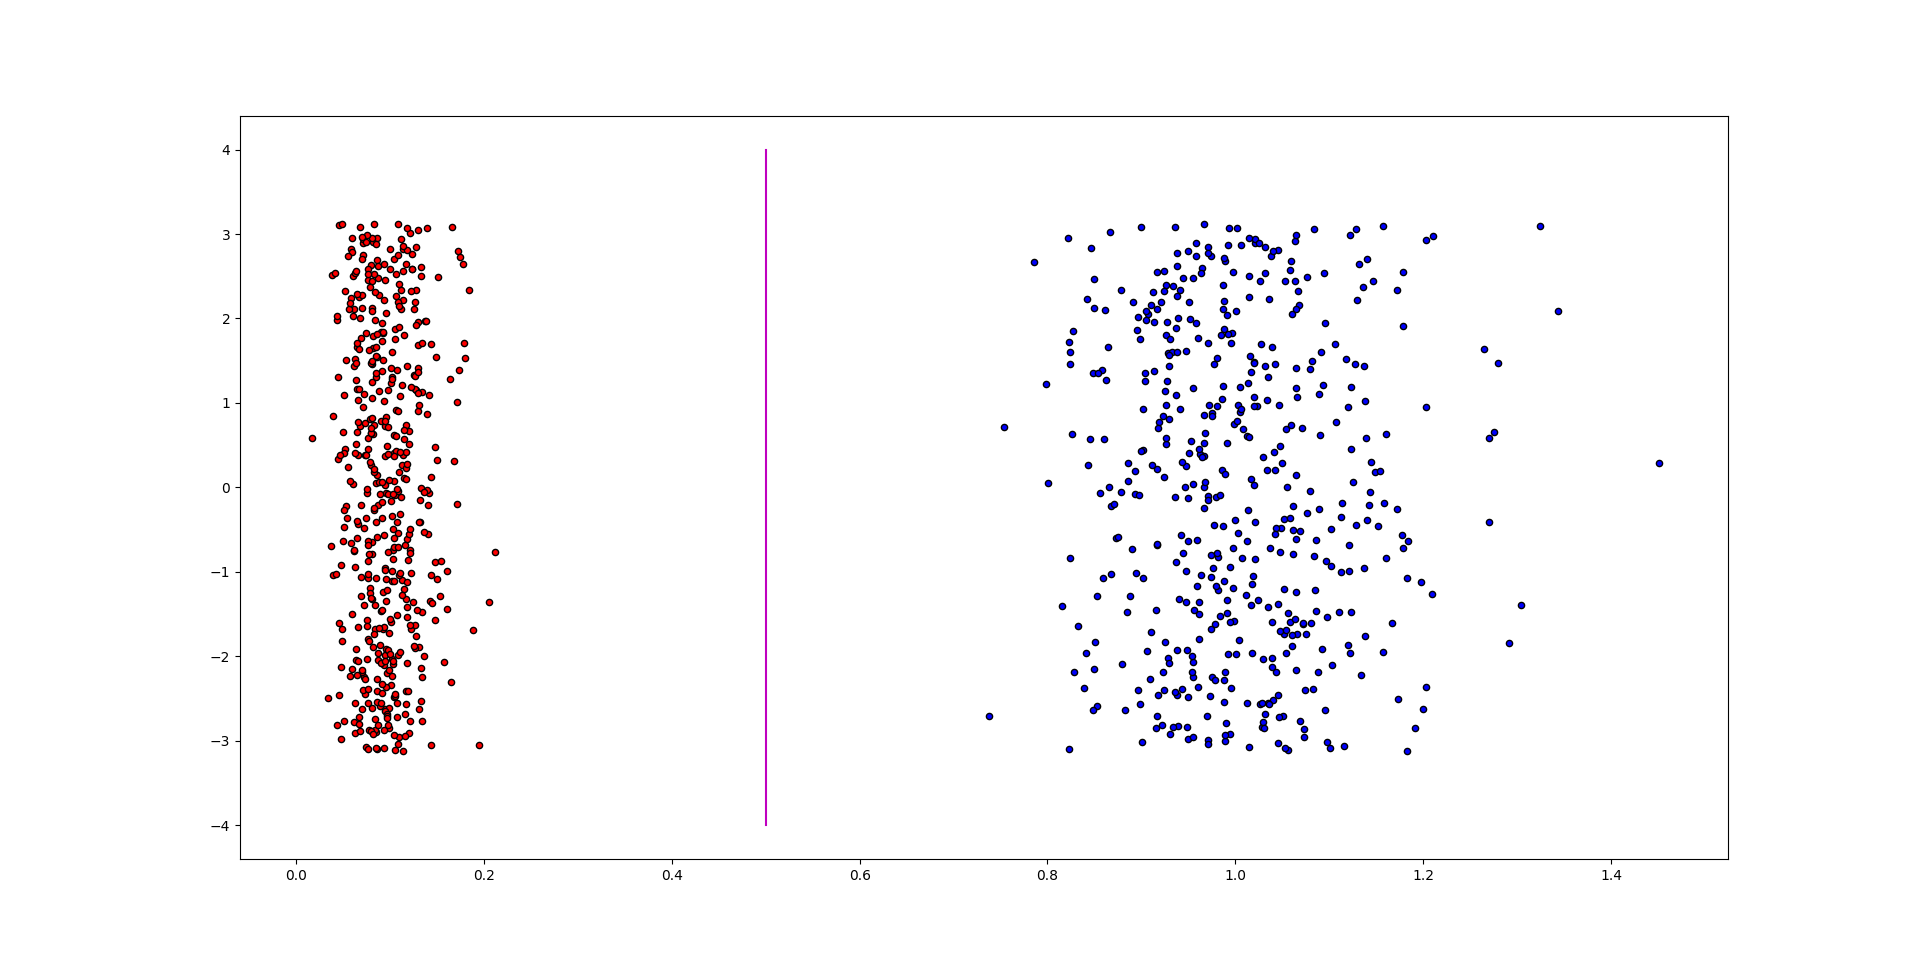
\includegraphics[width=.7\textwidth]{images/samples/separation_pol}
				\caption{\label{fig::kernel_polar} Exemple de changement d'espace avec une transfomation $\Phi$.}
			\end{figure}
			\item[--] \begin{align*}
				\Phi: \mathbb{R}^2 &\rightarrow \mathbb{R}^2 \\
				\begin{pmatrix}
					x \\
					y
				\end{pmatrix} &\mapsto \begin{pmatrix}
					x^2 + y^2 \\
					\arctan(x/y)
				\end{pmatrix}
			\end{align*}
		\end{itemize}
	\end{frame}
	\begin{frame}{Changement d'espace}
		\begin{itemize}
			\item[--] Trouver la transformation $\Phi$:
			\begin{figure}[H]
				\ffigbox[\FBwidth]
				{
					\begin{subfloatrow}[2]
						\ffigbox[\FBwidth]
						{
							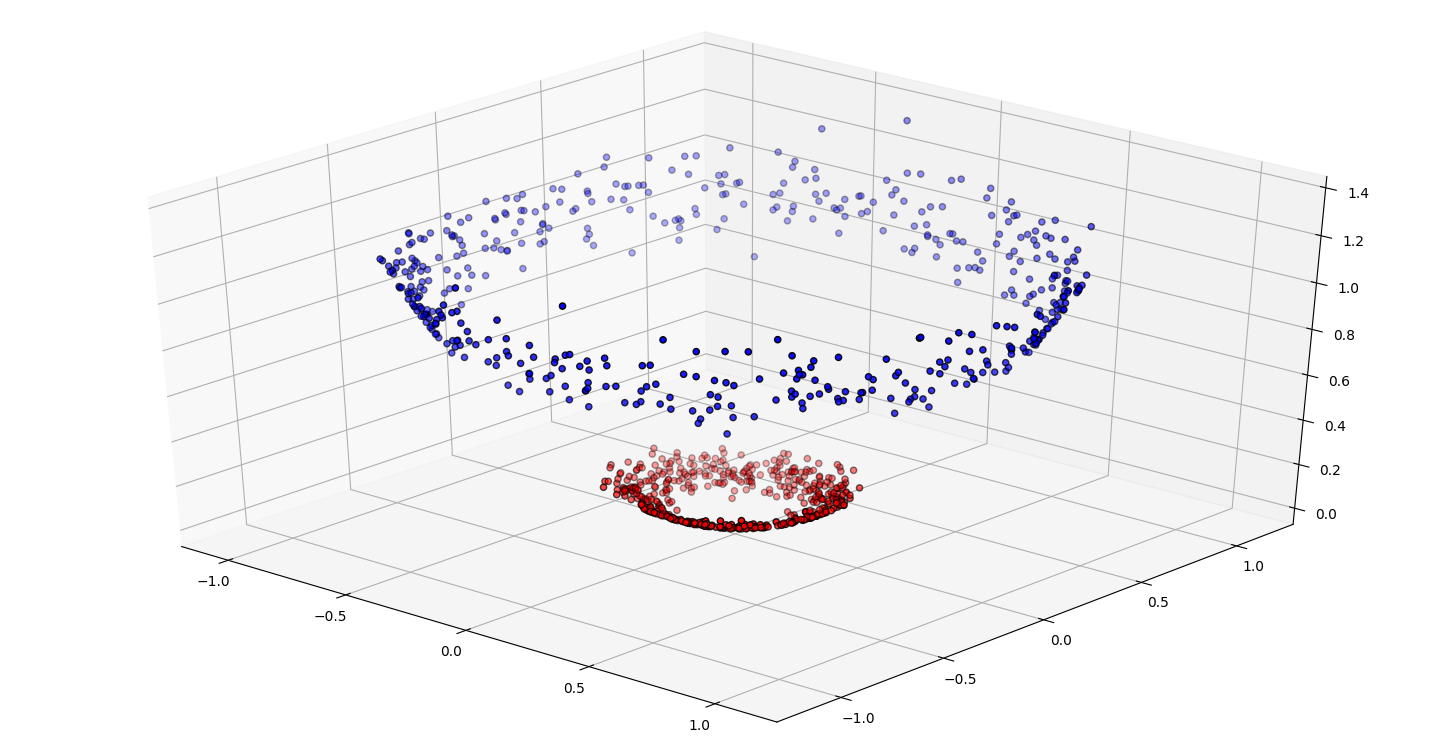
\includegraphics[width=.45\textwidth]{images/samples/map_L_2_separation_1}
						}
						{
							\caption{Vue de haut.}\label{fig::mano_take_1}
						}
						\ffigbox[\FBwidth]
						{
							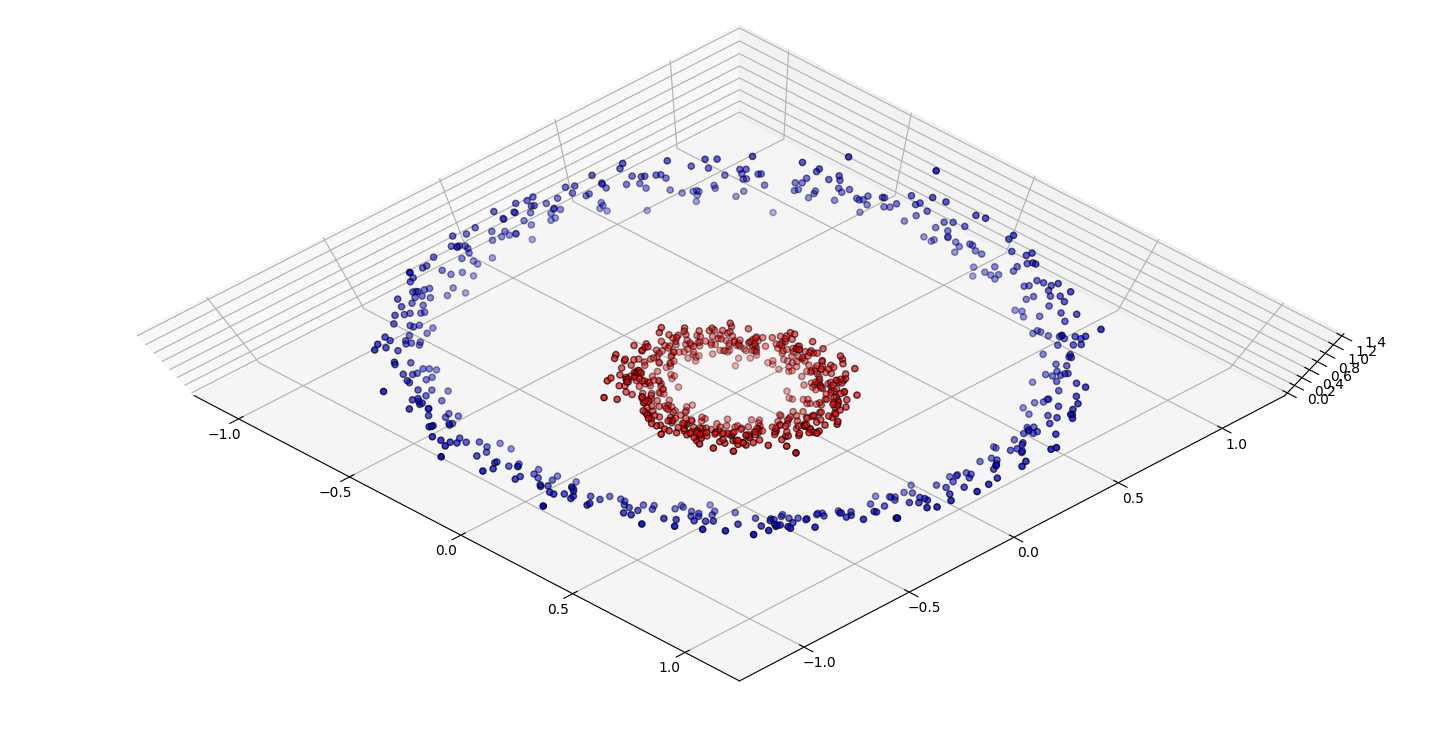
\includegraphics[width=.45\textwidth]{images/samples/map_L_2_separation}
						}
						{
							\caption{Vue transversale.}\label{fig::mano_take_2}
						}
					\end{subfloatrow}
				}
				{
					\caption{\label{fig::kernel_a_la_mano}  Exemple de changement d'espace avec une transfomation $\Phi$.}
				}
			\end{figure}
		\end{itemize}
	\end{frame}
	\begin{frame}{Changement d'espace}
		\begin{itemize}
			\item[--]<1-> Séparation linéaire dans le nouveau espace:
			\begin{figure}[H]
				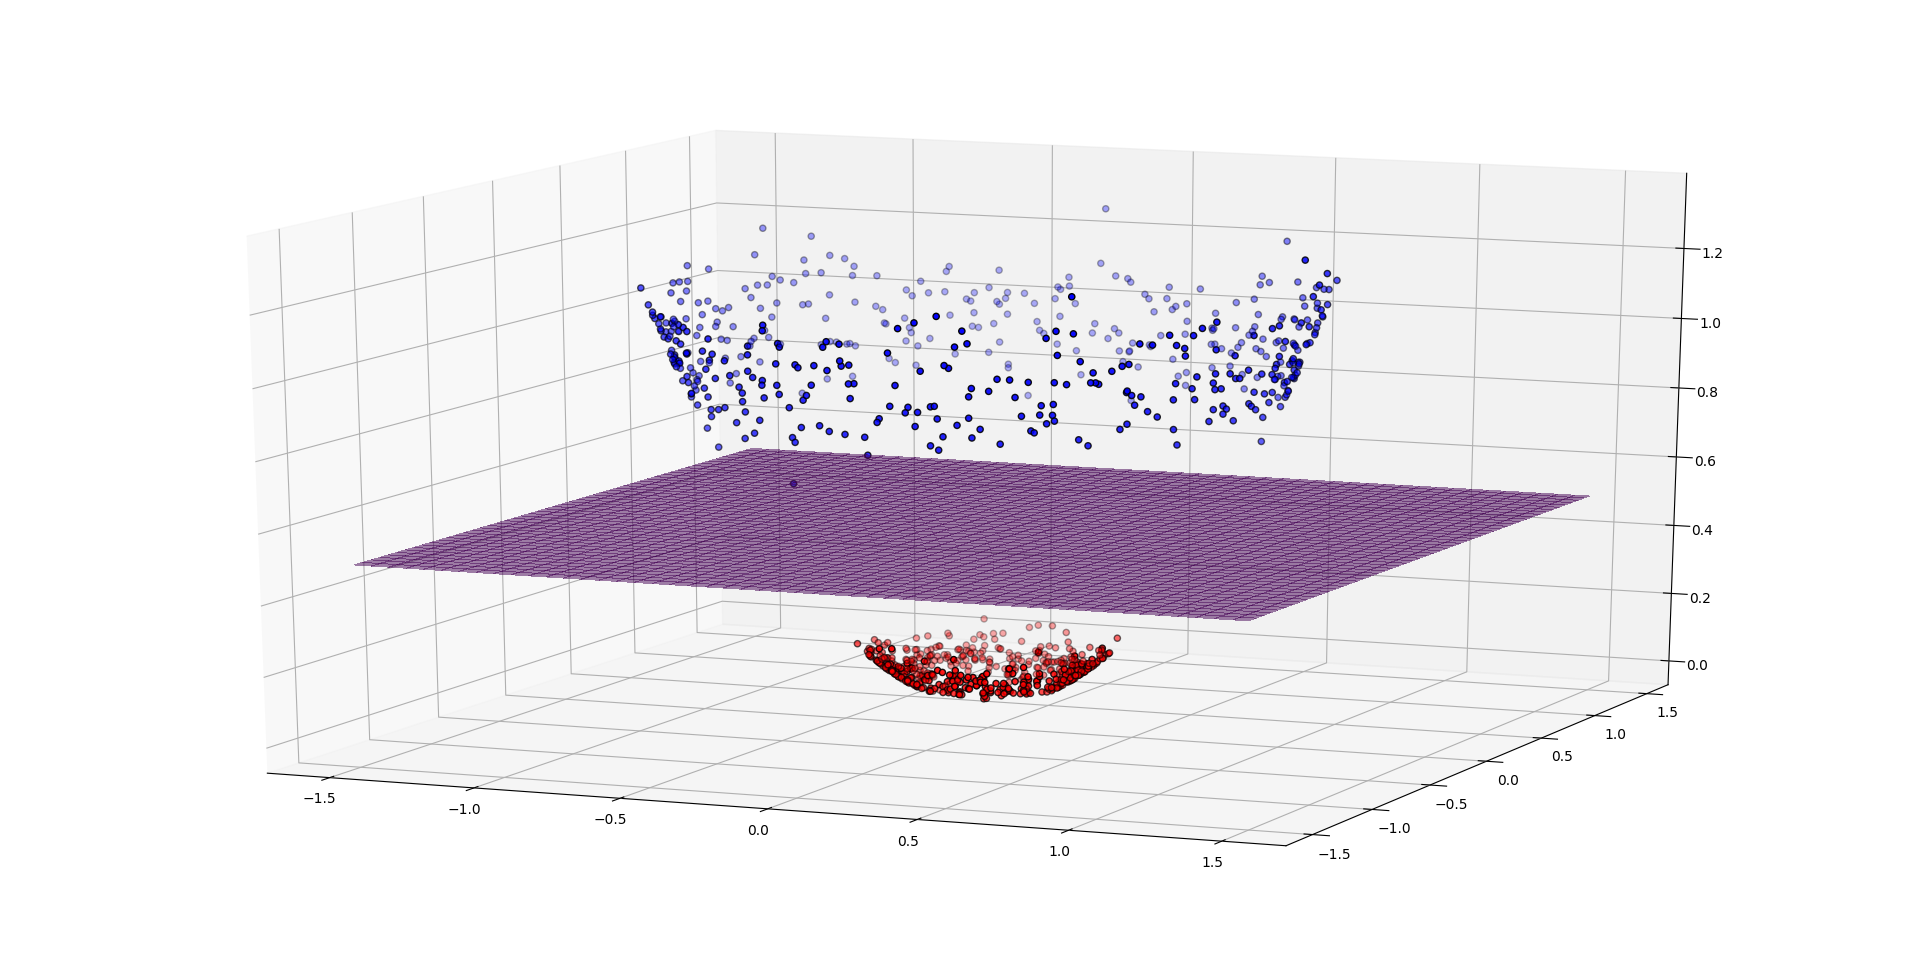
\includegraphics[width=.5\textwidth]{images/samples/separation_x_2_y_2}
				\caption{\label{fig::mano_take_3} Hyperplan séparant les deux classes dans le nouveau espace.}

			\end{figure}
			\item[--]<2-> \begin{align*}
				\Phi: \mathbb{R}^2 &\rightarrow \mathbb{R}^3 \\
				\begin{pmatrix}
					x \\
					y
				\end{pmatrix} &\mapsto \begin{pmatrix}
					x \\
					y \\
					x^2 + y^2
				\end{pmatrix}
			\end{align*}
		\end{itemize}
	\end{frame}
	\begin{frame}{Changement d'espace}
		\begin{itemize}
			\item[--] Trouver la transformation $\Phi$:
			\begin{figure}[H]
				\ffigbox[\FBwidth]
				{
					\begin{subfloatrow}[2]
						\ffigbox[\FBwidth]
						{
							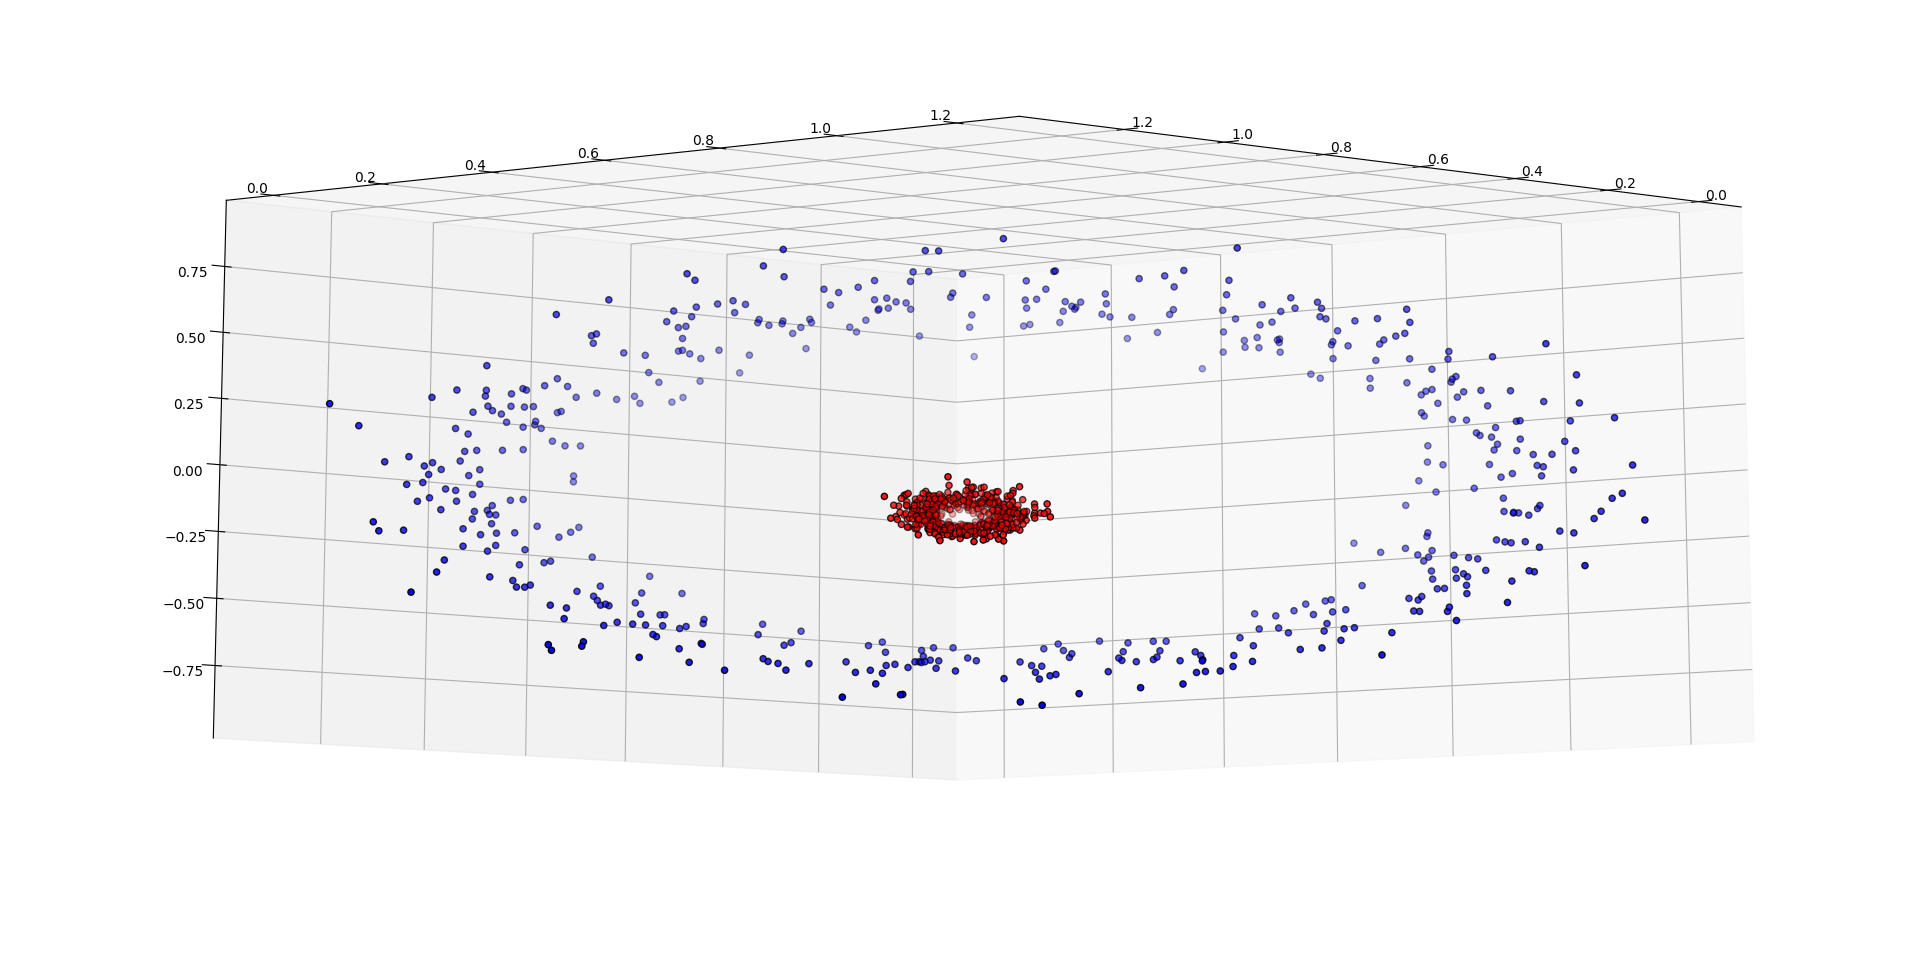
\includegraphics[width=.45\textwidth]{images/samples/separation_pol_2_1}
						}
						{
							\caption{Vue de haut.}\label{fig::pol_take_1}
						}
						\ffigbox[\FBwidth]
						{
							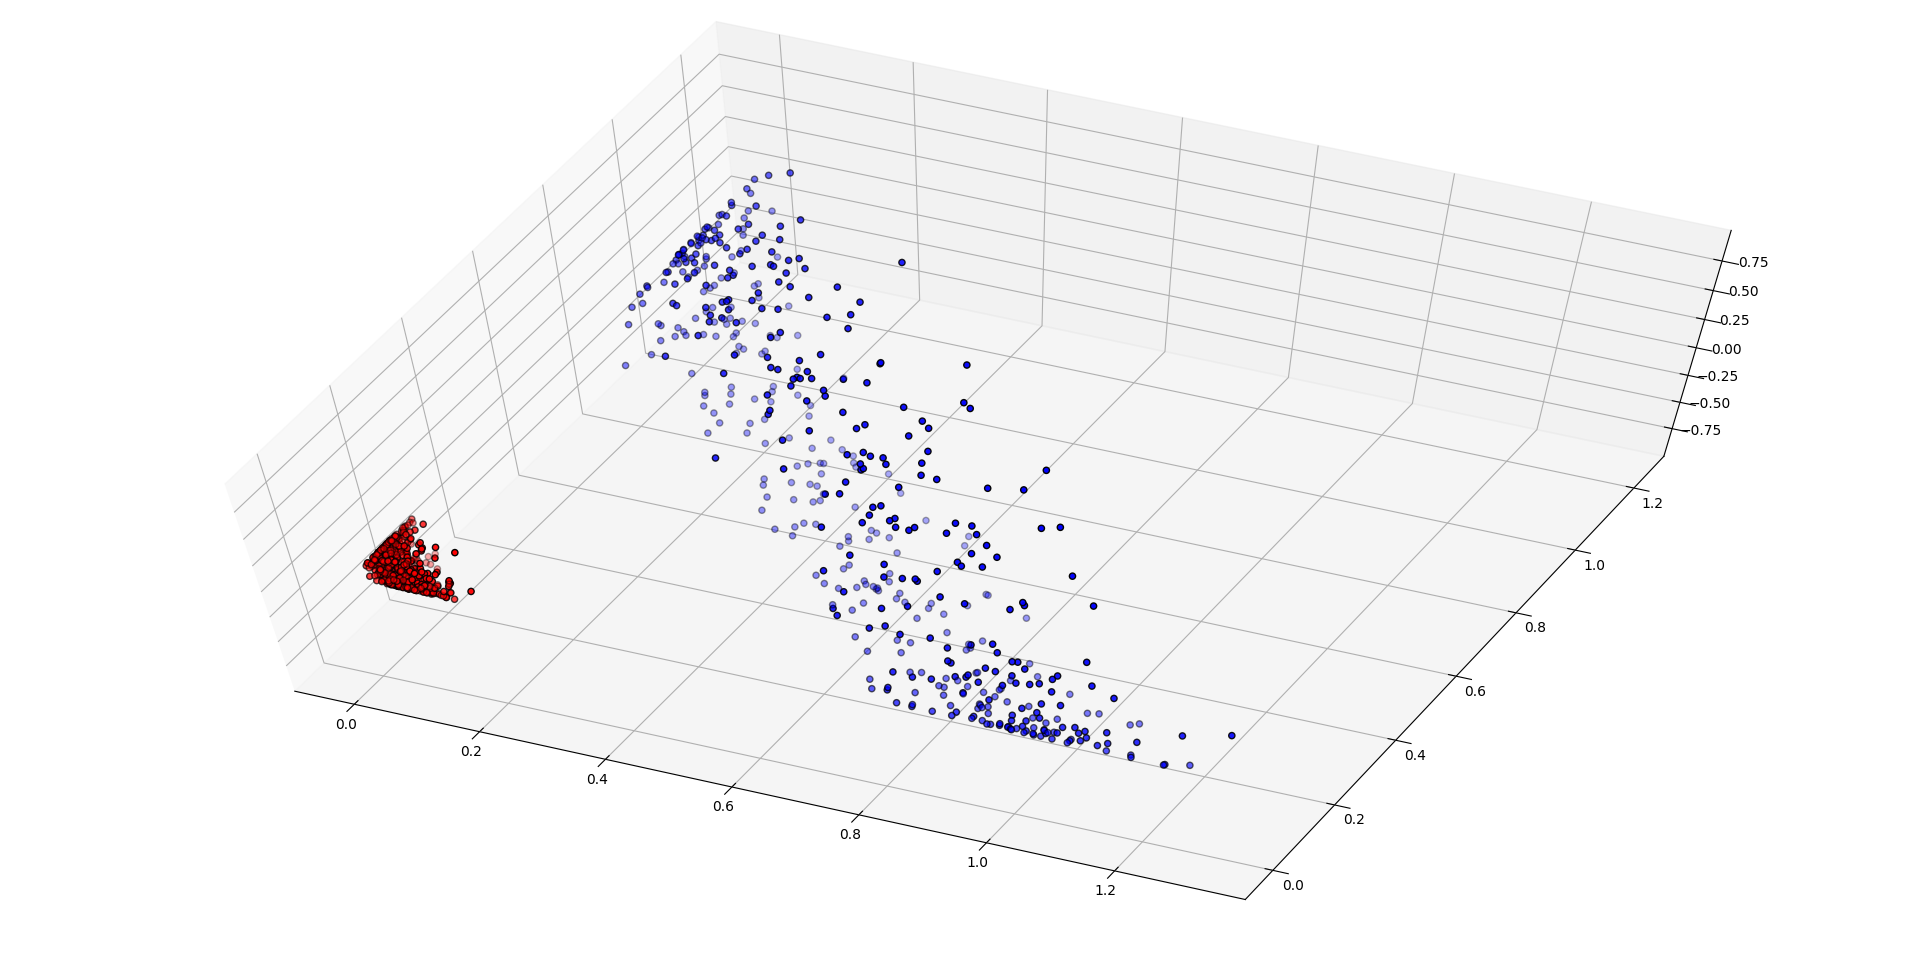
\includegraphics[width=.45\textwidth]{images/samples/separation_pol_2_2}
						}
						{
							\caption{Vue transversale.}\label{fig::pol_take_2}
						}
					\end{subfloatrow}
				}
				{
					\caption{\label{fig::kernel_poly}  Exemple de changement d'espace avec une transfomation $\Phi$.}
				}
			\end{figure}
		\end{itemize}
	\end{frame}
	\begin{frame}{Changement d'espace}
		\begin{itemize}
			\item[--]<1-> Séparation linéaire dans le nouveau espace:
			\begin{figure}[H]
				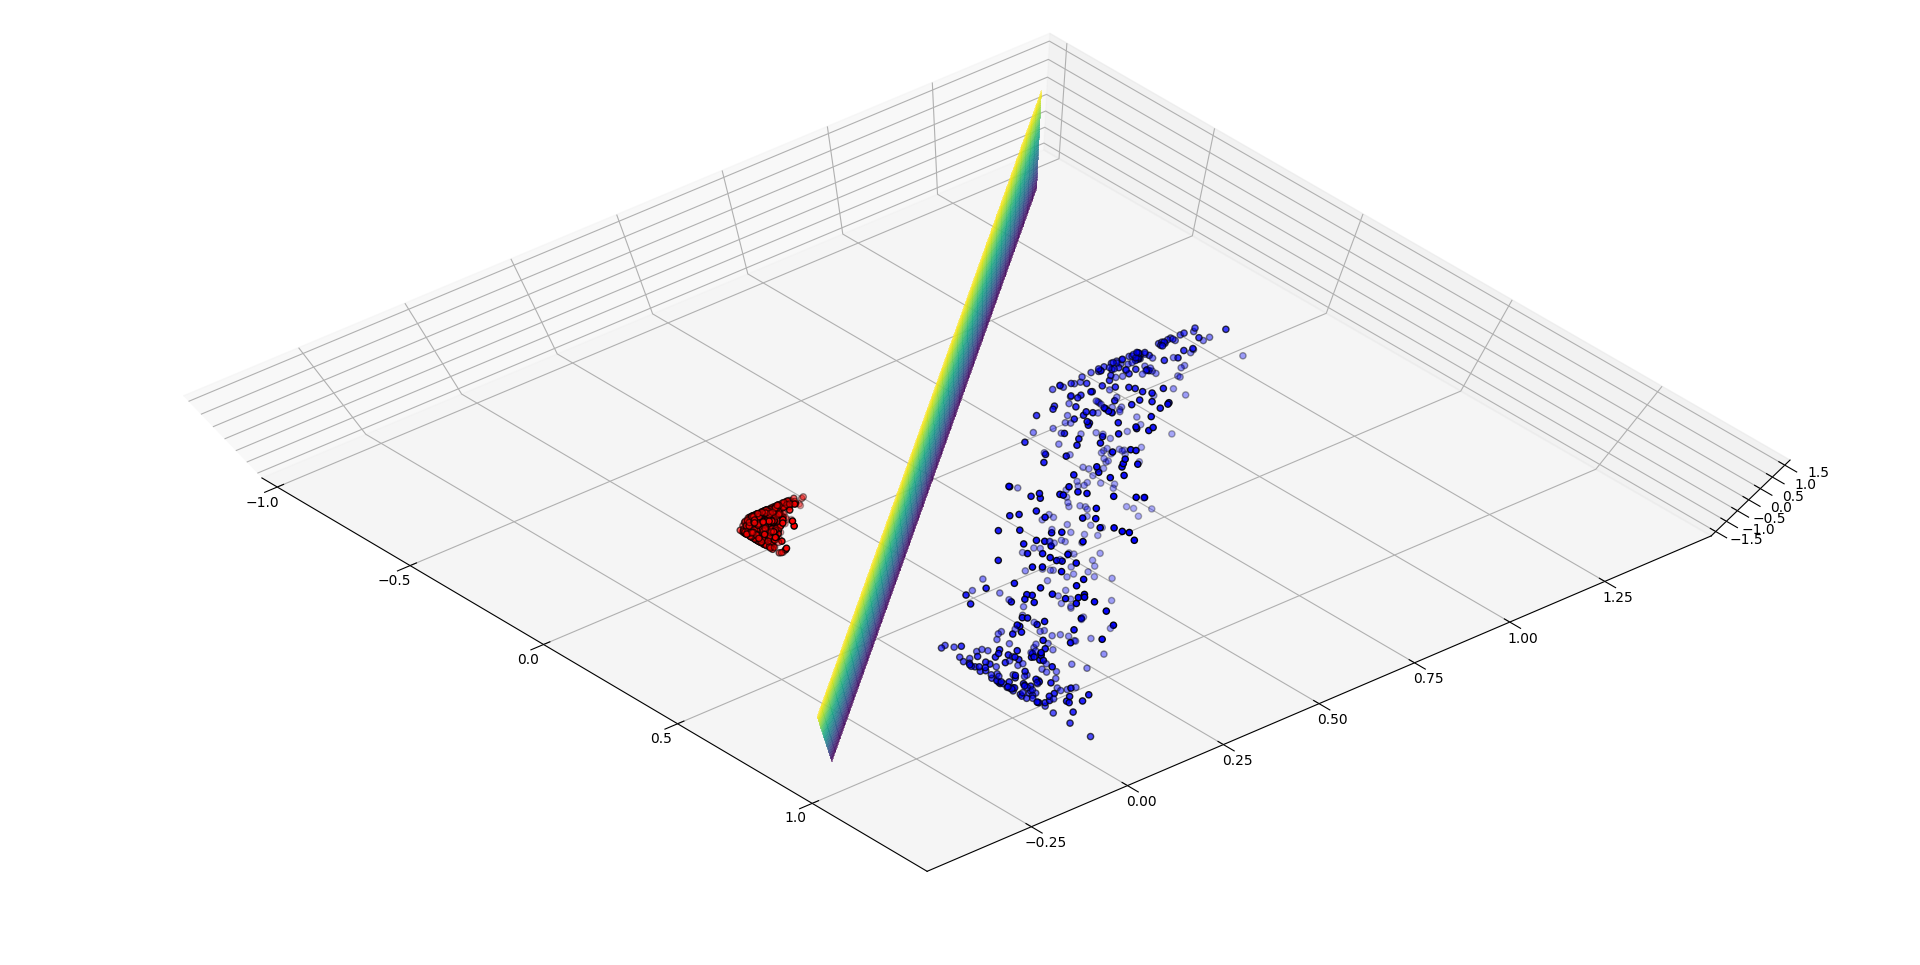
\includegraphics[width=.7\textwidth]{images/samples/separation_pol_2_3}
				\caption{\label{fig::pol_take_3} Hyperplan séparant les deux classes dans le nouveau espace.}

			\end{figure}
			\item[--]<2-> \begin{align*}
				\Phi: \mathbb{R}^2 &\rightarrow \mathbb{R}^3 \\
				\begin{pmatrix}
					x \\
					y
				\end{pmatrix} &\mapsto \begin{pmatrix}
					x^2 \\
					y^2 \\
					\sqrt{2}.x.y
				\end{pmatrix}
			\end{align*}
		\end{itemize}
	\end{frame}
	\begin{frame}{Changement d'espace}
		\begin{itemize}
			\item[--] Le but du changement d'espace est de pouvoir séparer linéairement le problème dans un nouveau espace où les distances Euclidiennes ont un sens;
			\item[--] On transforme donc les instances avec une application comme suit:
			\begin{align*}
				\Phi: \mathbb{R}^d &\rightarrow \mathbb{R}^p \\
				X &\mapsto \Phi(X)
			\end{align*}
			où $p\geq d$.
		\end{itemize}
	\end{frame}

	\begin{frame}{Que devient donc le problème d'optimisation:}
		\begin{itemize}
			\item[--] Problème primal:
			\begin{equation}
				\begin{aligned}
				& \min_{\textbf{w}, \xi_1,\dots,\xi_n \in \mathbb{R}^+}
				& & {\vert\vert \textbf{w} \vert\vert}^2 + C.\sum_{i=1,\dots,n}\xi_i \\
				& \text{sous contrainte}
				& & Y^i.(\textbf{w}.\Phi(\textbf{X}^i) + b) \geq 1 - \xi_i , \forall i = 1, \dots, n.
				\end{aligned}
			\end{equation}
			\item[--] Problème dual:
			\begin{equation}
				\begin{aligned}
				& \max_{0 \leq \alpha_i \leq C ,\forall i=1,\dots,n}
				& & \sum_{i=1,\dots,n} \alpha_i - \frac{1}{2}.\sum_{l,p=1,\dots,n}\alpha_l.\alpha_p.Y^l.Y^p.(\Phi(X^l).\Phi(X^p))\\
				& \text{sous contrainte}
				& & \sum_{i=1,\dots,n}Y^i.\alpha_i=0
				\end{aligned}
			\end{equation}
			\item[--] Que peut on relever sur ce dernier problème d'optimisation?
		\end{itemize}
	\end{frame}

	\begin{frame}{Kernel Trick}
		\begin{itemize}
			\item[--]<1-> La transformation $\Phi$ ne nous intéresse pas, en soi;
			\item[--]<2-> Ce sont les distances Euclidienne dans le nouveau espace:
			$$\forall X, Y \in \mathbb{R}^d$$
			\begin{align*}
				\vert\vert\Phi(X) - \Phi(Y)\vert\vert_2^2 &= \vert\vert\Phi(X)\vert\vert_2^2 + \vert\vert\Phi(Y)\vert\vert_2^2 - 2 \vert\vert\Phi(X)\vert\vert.\vert\vert\Phi(Y)\vert\vert_2^2 \\
				 &= {\Phi(X)}^t.\Phi(X) + {\Phi(Y)}^t.\Phi(Y) - 2 {\Phi(X)}^t.\Phi(Y)
			\end{align*}
			\item[--]<3-> Il suffit de calculer le nouveau produit scalaire:
			\begin{equation}
				\forall X, Y \in \mathbb{R}^d \quad k(X, Y) \triangleq {\Phi(X)}^t.\Phi(Y)
			\end{equation}
			où:
			\begin{align*}
				k: \mathbb{R}^d \times \mathbb{R}^d &\rightarrow \mathbb{R}^+ \\
				(X, Y) &\mapsto k(X, Y)
			\end{align*}
			est ce qu'on appelle le \textit{kernel}.
		\end{itemize}
	\end{frame}

	\begin{frame}{Kernels Usuels}
		\begin{itemize}
			\item[--] Radial Basis Function (RBF):
			\begin{equation}
				k_{\gamma}(x,y) = \exp{-\gamma.\vert\vert x-y \vert\vert^2}
			\end{equation}
			\item[--] Kernel Polynomial:
			\begin{equation}
				k_{\gamma, c}(x,y) = (x^t.y + c)^{\gamma}
			\end{equation}
			\item[--] Kernel Sigmoidal:
			\begin{equation}
				k_{\gamma, c}(x,y) = \gamma.\tanh(x^t.y + c)
			\end{equation}
		\end{itemize}
	\end{frame}

	\begin{frame}{Kernels Usuels}
		\begin{figure}[H]
			\ffigbox[\FBwidth]
			{
				\begin{subfloatrow}[2]
					\ffigbox[\FBwidth]
					{
						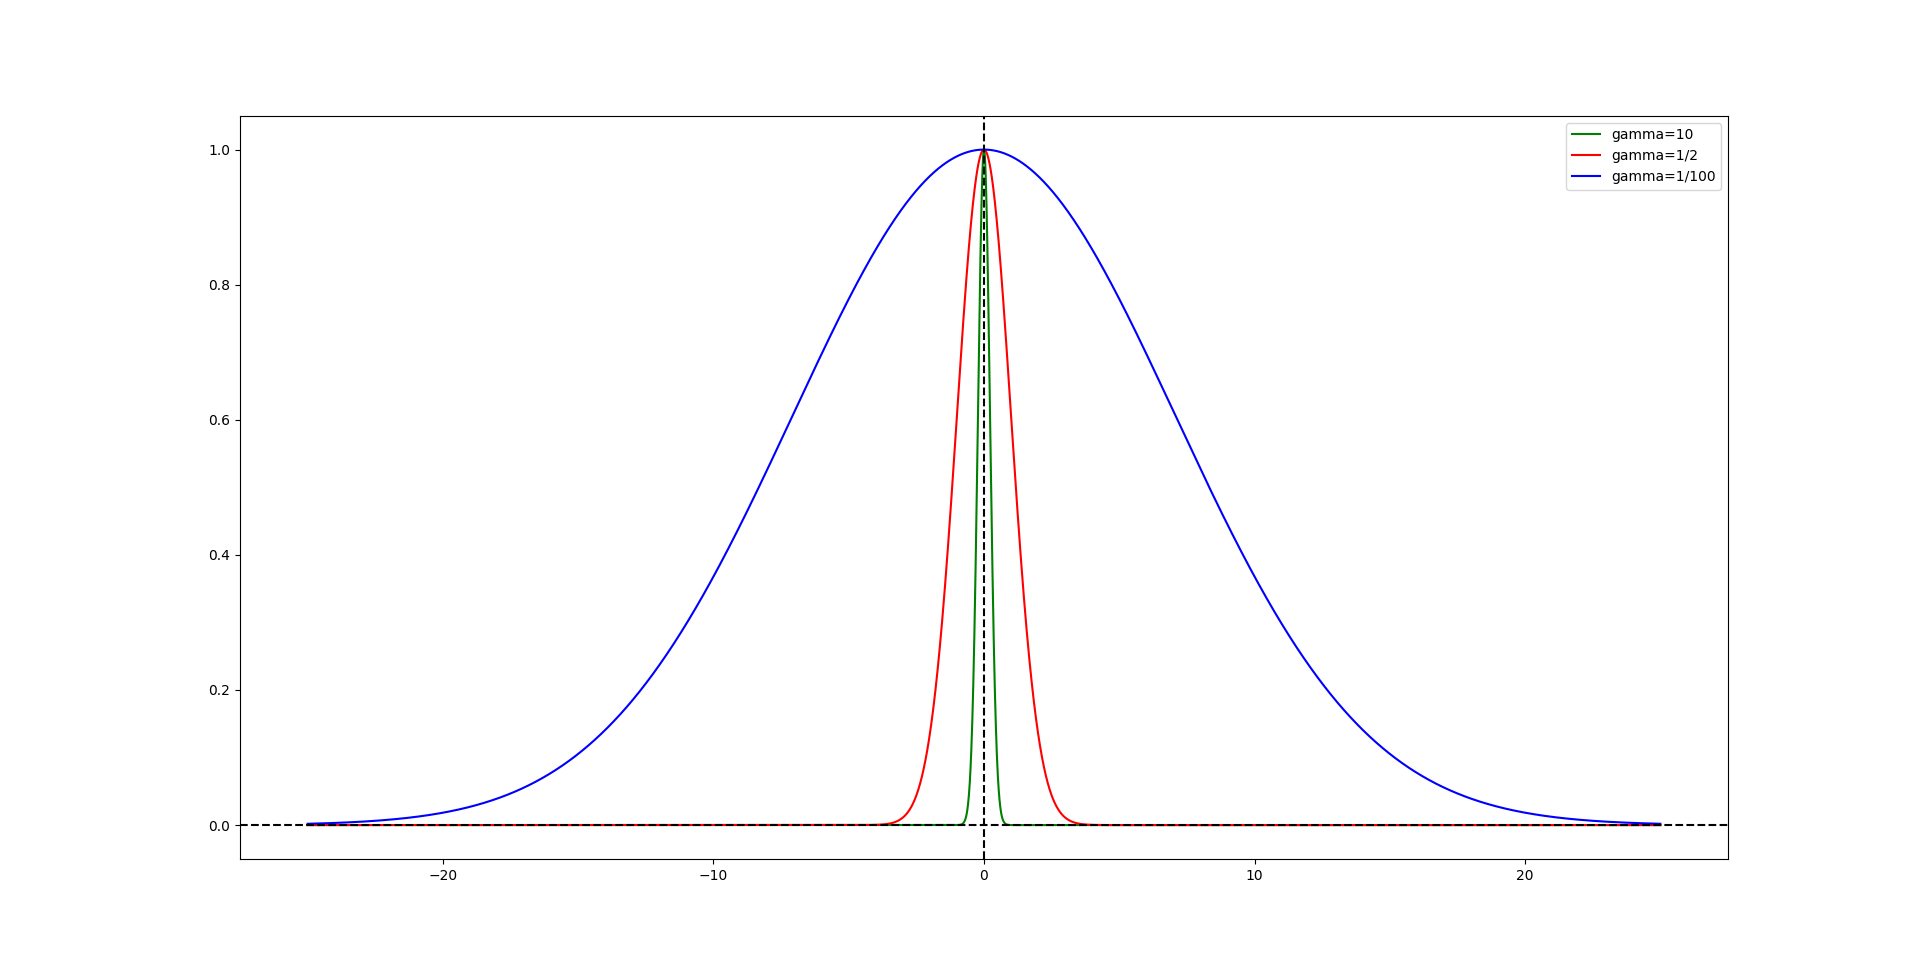
\includegraphics[width=.45\textwidth]{images/samples/rbfs}
					}
					{
						\caption*{RBF avec différentes valeurs de $\gamma$.}\label{fig::rbfs}
					}
					\ffigbox[\FBwidth]
					{
						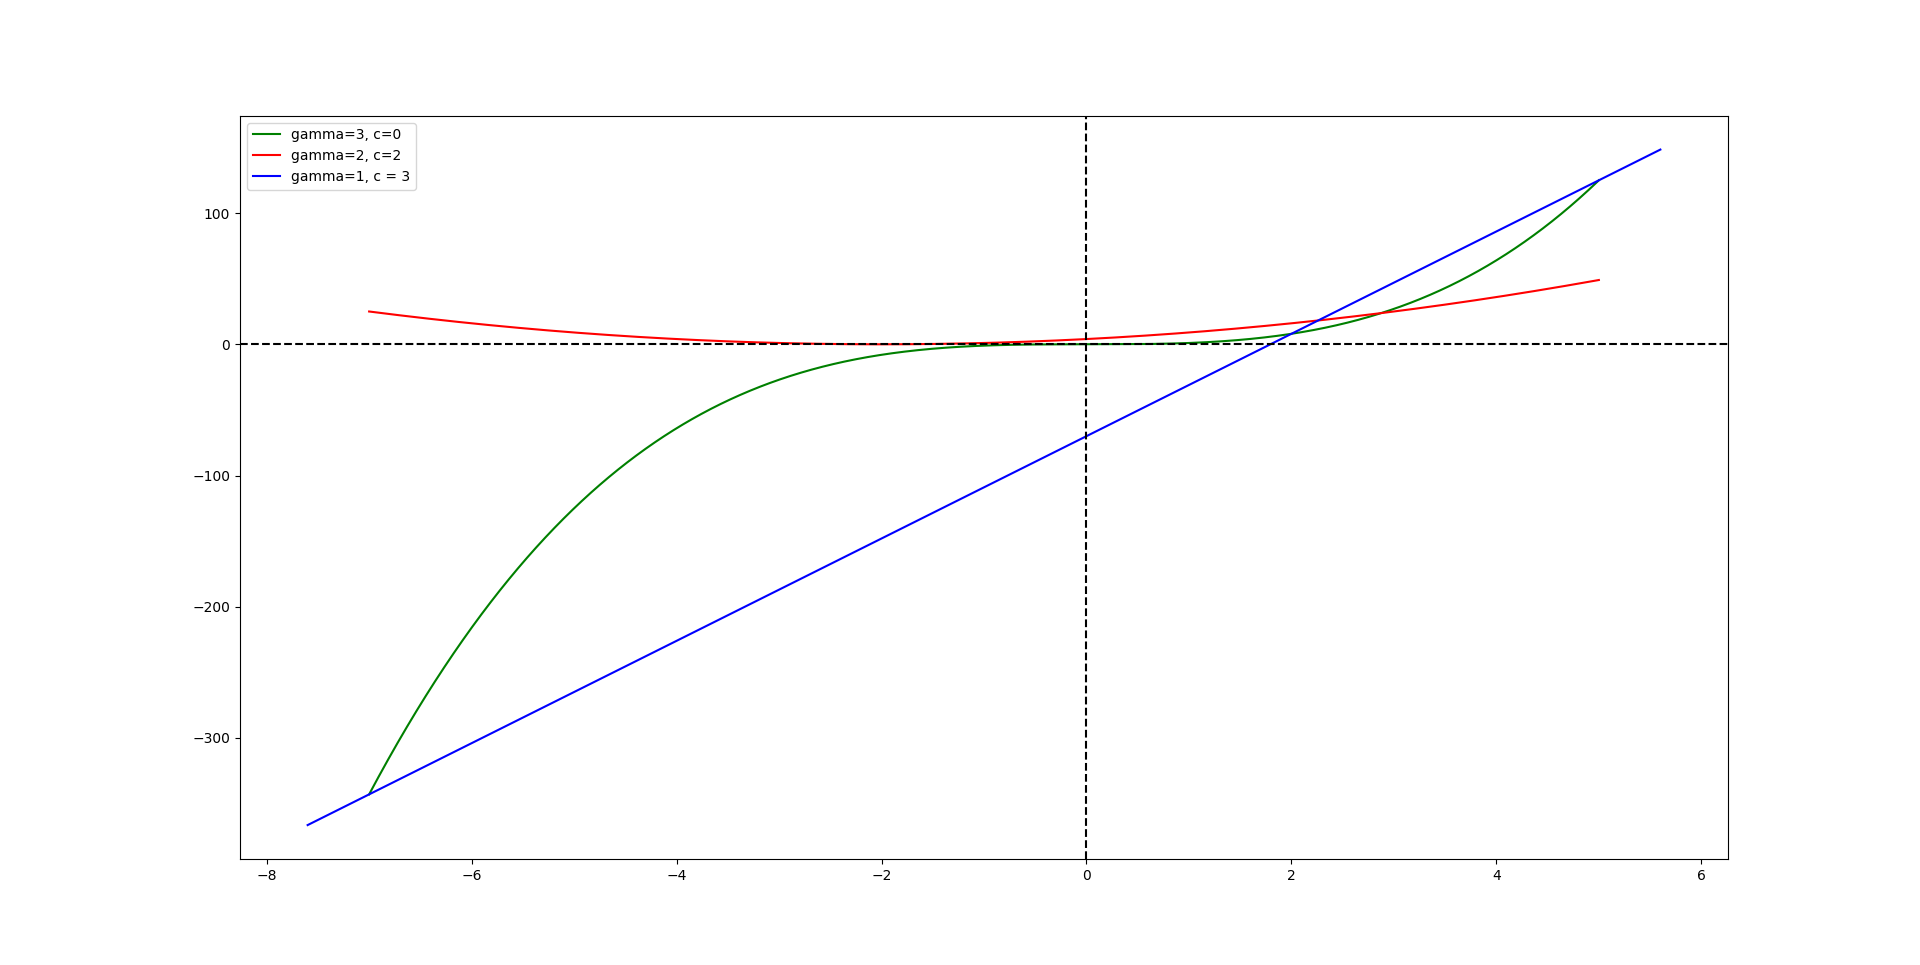
\includegraphics[width=.45\textwidth]{images/samples/polys}
					}
					{
						\caption*{Kernels Polynomiaux avec différentes valeurs de $\gamma$ et $c$.}\label{fig::polys}
					}
				\end{subfloatrow}
			}
			{
				\caption*{}
			}
			\ffigbox[\FBwidth]
			{
				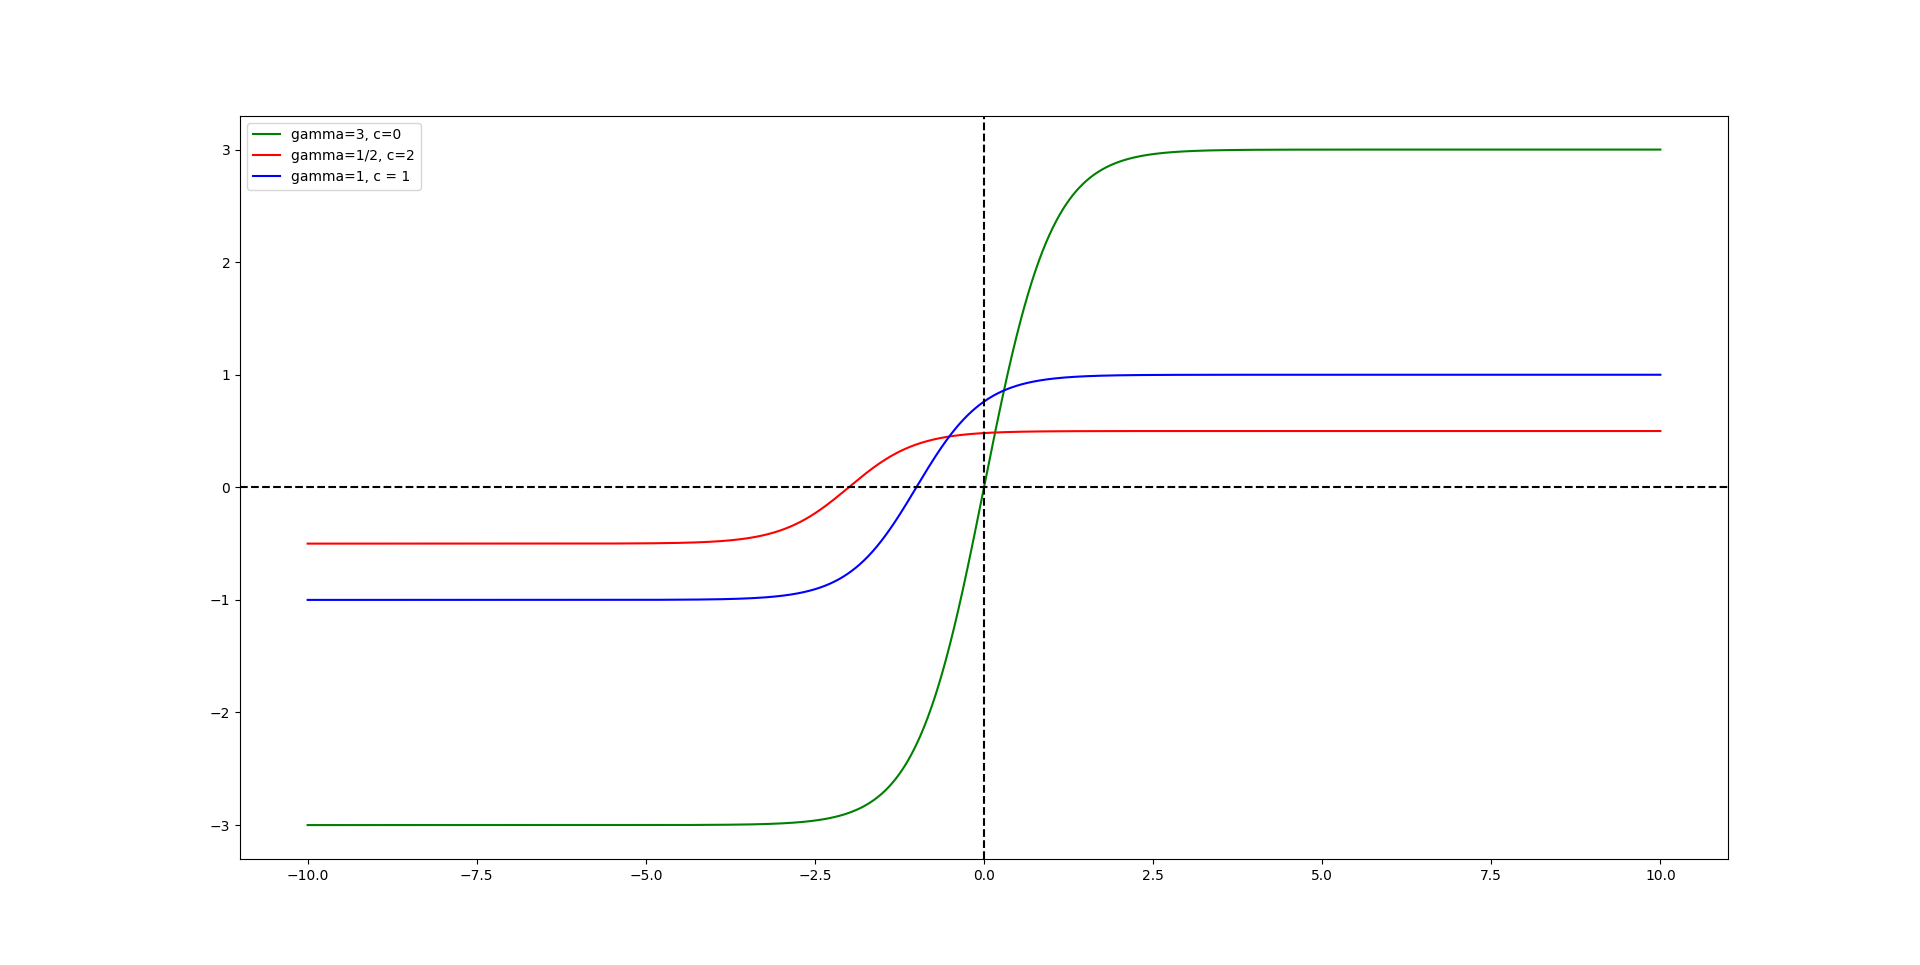
\includegraphics[width=.5\textwidth]{images/samples/tanhs}
			}
			{
				\caption*{Kernels Sigmoids avec différentes valeurs de $\gamma$ et $c$.}\label{fig::tanhs}
			}
		\end{figure}
	\end{frame}

	\section[feature selection]{Sélection d'attributs}
	\subsection[motivation]{Motivation}
	\begin{frame}{Pourquoi sélectionner les attributs?}
		Les espaces à très grande dimension ne resemble pas au plan ou au volume:
		\begin{itemize}
			\item[--]<1-> Les calculs durent plus de temps,
			\item[--]<2-> Il y a moins de volume à l'intérieur; si on compare le volume contenu dans une sphère et le volume de l'hypercube circonscrit:
			$$\frac{V(\mathbb{B}_{2}(r))}{V(\mathbb{B}_{\infty}(r))}\xrightarrow[d \to \infty]{} 0$$
			\item[--]<3-> La distance Euclidienne n'a plus de sens en très grande dimension $\longrightarrow$ moins d'attributs on a mieux sont les résultas~\cite{Domingos:2012:FUT:2347736.2347755}.
		\end{itemize}
	\end{frame}

	\begin{frame}{Comment sélectionner les attributs?}
		Encore un fois, sans connaissance préalable, la sélection d'attributs est insoluble vue le nombre exponentiel de possibilité $\sum_{k=0,\dots,n} \begin{pmatrix}
		n\\
		k
		\end{pmatrix} = 2^n$.

		On distingue donc trois types d'approche:
		\begin{enumerate}
			\item<1-> approche par filtre: on choisit les attributs en amont en reposant sur un critère,
			\item<2-> approche intégrée: on sélectionne les attributs en reposant sur les caractéristiques du classifieur,
			\item<3-> approche symbiotique: on retient les attributs les plus performants en aval.
		\end{enumerate}
	\end{frame}

	\subsection[filter approach]{Approche par filtre}
	\begin{frame}{Approche par filtre}
		\begin{itemize}
			\item[--] Corrélation: un bon sous-ensemble contient des attributs pas très corrélés entre eux $\longrightarrow$ on élimine les variables redondantes;
			\item[--] Relief: qualification d'un attribut en fonction de comment ses valeurs permettent de distinguer des points qui sont proches.
		\end{itemize}
	\end{frame}

	\subsection[integrated approach]{Approche intégrée}
	\begin{frame}{Approche intégrée: cas du SVM-RFE}
		On repose par exemple sur les poids du SVM $ --- i.e. \textbf{w}$:
		\begin{enumerate}
			\item<1-> On entraine le SVM $\longrightarrow$ on obtient le $\textbf{w}$.
			\item<2-> On choisit l'attribut $i$ avec le plus faible poids:
			$$ i \leftarrow \arg \min_{k=1,\dots,d}{\vert\vert w_k\vert\vert}$$
			\item<3-> On élimine l'attribut $i$.
		\end{enumerate}
		On procède donc par récurrence jusqu'au nombre d'attributs cherché~\cite{Guyon2002}.
	\end{frame}

	\subsection[symbiotic approach]{Approche symbiotique}
	\begin{frame}{SFS}
		Sélection ascendante (SFS\@: Sequential Forward Selection).
		\begin{enumerate}
		\item<1-> On sélectionne le meilleur attribut;
		\item<2-> On lui rajoute l'attribut qui forme la meilleur paire;
		\item<3-> On continue à rajouter les attributs de manière à avoir à l'itération $k$ le meilleur $k$-tuple;
		\item[--]<4-> Le problème est que l'on peut rater en procédant ainsi au meilleur ensemble.
		\end{enumerate}
	\end{frame}

	\begin{frame}{SFS}
		\begin{block}{Exemple}
			\begin{center}
				\begin{longtable}{c c c c c}
					\toprule
					attributs sélectionés & $1$ & $2$ & $3$ & $4$\\
					\midrule
					résultat& $0.49$ & $0.21$ & $0.19$ &$0.24$\\
					\bottomrule
				\end{longtable}
				\begin{longtable}{c c c c c c c}
					\toprule
					attributs sélectionés & $1,2$ & $1,3$ & $1,4$ & $2,3$ & $2,4$ & $3,4$\\
					\midrule
					résultat & $0.59$ & $0.51$ & $0.52$ & $0.45$ & $0.49$ & $0.48$\\
					\bottomrule
				\end{longtable}
				\begin{longtable}{c c c c c c c}
					\toprule
					attribut sélectionés & $1,2,3$ & $1,2,4$ & $1,3,4$ & $2,3,4$ & $1,2,3,4$\\
					\midrule
					résultat & $0.61$ & $0.67$ & $0.59$ & $0.78$ & $0.81$\\
					\bottomrule
				\end{longtable}
			\end{center}
		\end{block}
	\end{frame}

	\begin{frame}{SBE}
		Sélection descendante (SBE\@: Sequential Backward Elimination).
		Cette méthode ressemble à celle d'avant.
		\begin{enumerate}
		\item<1-> On élimine le attribut qui ne rapporte pas beaucoup;
		\item<2-> On réitère de façon à ce que qu'à l'itération $k$ on aura éleminé les $k$ pire attribut;
		\item<3-> On continue jusqu'à ce qu'il ne reste plus qu'un attribut ou un nombre donné.
		\item[--]<4-> On rencontre le même problèmes qu'avant.
		\end{enumerate}
	\end{frame}

	\begin{frame}{Comment résoudre le problème donc?}
		\begin{itemize}
			\item<1-> Combinaison SFS + SBE\@: sélection Plus-L-Moins-R\@:
			\begin{itemize}
				\item Si $L > R$, on commence avec un ensemble vide, on ajoute L attributs puis on en enlève R\@,
				\item Si $L < R$, on commence avec tous les attributs, on enlève R attributs puis on en rajoute L\@;
			\end{itemize}
			\item<2-> On garantit la convergence vers une solution unique:
			\begin{itemize}
				\item On peut vérifier que SFS et SBE ne se contredisent pas.
				\item On peut procéder comme dans l'exemple:
				\begin{block}{Exemple}
					Si SFS veut ajouter un attribut, il vérifie qu'il n'a pas été éliminé par SBE\@. Si oui, il prend le 2$^{\text{ème}}$ meilleur et ainsi de suite.
				\end{block}
			\end{itemize}
		\end{itemize}
	\end{frame}

	\section{Références}
	\begin{frame}[allowframebreaks]{Références}
		\nocite{sklearn_api}
		\nocite{camps2009kernel}
		\nocite{CC01a}
		\bibliographystyle{apalike}
		\bibliography{references.bib}
	\end{frame}

\end{document}
